%!TEX program = xelatex
\documentclass[a4paper,12pt,openany,twoside]{book} % twoside
\usepackage[inner=3.5cm,outer=2.5cm, top=2.5cm]{geometry} %showframe

\usepackage{url}
\usepackage{fontspec}
\usepackage{lmodern}
\usepackage{csquotes}
\usepackage{graphicx}
\usepackage{caption}
\usepackage{subcaption}
\usepackage[rgb]{xcolor}
\graphicspath{ {assets/} }
\usepackage{xunicode}
\usepackage{xltxtra}
\usepackage{chngcntr}
\usepackage[czech]{babel}
\usepackage[pagestyles,medium]{titlesec}
\usepackage{setspace}
\usepackage{emptypage}
\usepackage{xpatch}
\usepackage{caption}
\usepackage{subcaption}
\usepackage{ragged2e}
\usepackage{pbox}
\usepackage{rotating}
\usepackage{float}
\usepackage{afterpage}
\usepackage{tipa}

\usepackage[hidelinks]{hyperref}

\usepackage{mdframed}
\usepackage{framed}
\def\tightlist{}

\xpatchcmd{\part}{\thispagestyle{plain}}{\thispagestyle{empty}}{}{}


\newcommand\exmp{\textsf}

\counterwithout{figure}{chapter}
\counterwithout{footnote}{chapter}


\newpagestyle{sensible}{
	\headrule\sethead{}{}{\MakeUppercase{\chaptertitle}}
	\setfoot{}{\thepage}{}
}

\setlength\emergencystretch{1em}
\setlength\headheight{14pt}
\setstretch{1.1}
\setcounter{secnumdepth}{4}

\widowpenalty10000
\clubpenalty10000

\hyphenation{выпа-дений}

\setmainfont[Ligatures=TeX]{CMU Serif Roman}

\usepackage[backend=biber, style=iso-authoryear, sortlocale=cs\_CZ, uniquelist=false, autocite=footnote, maxcitenames=2, maxbibnames=99, minnames=1, urldate=long, spacecolon=false,bibencoding=UTF8
]{biblatex}
\let\oldmultinamedelim\multinamedelim
\let\oldfinalnamedelim\finalnamedelim
\renewcommand*{\multinamedelim}{~a~}
\renewcommand*{\finalnamedelim}{~a~}
\renewcommand*{\nameyeardelim}{~}
\AtBeginBibliography{%
  \renewcommand*{\multinamedelim}{~--\space}%
  \renewcommand*{\finalnamedelim}{~--\space}%
}
\DefineBibliographyStrings{czech}{%
  mathesis = {Bakalářská diplomová práce},
  editors = {eds.}
}

\addbibresource{bibliography.bib}

\newcommand{\sign}[1]{%      
  \begin{tabular}[t]{@{}r@{}}
  \makebox[2.5in]{\dotfill}\\
  \strut#1\strut
  \end{tabular}%
}


\begin{document}
	\clearpage
	\pagenumbering{gobble}

	\begin{titlepage}
		\begin{center}
			{\Large\uppercase{Masarykova univerzita}}

			\vspace{1em}

			{\Large Filozofická fakulta}

			\vspace{1em}

			{\large Ústav českého jazyka}

			\vspace{1em}

			{\large Český jazyk se specializací počítačová lingvistika}

			\vspace{11em}

			{\large Kryštof Davídek }
			
			\vspace{3em}
			
			{\LARGE\bf Elektronický slovník s definicemi založenými na derivačních rysech slovotvorně motivovaných slov}

			\vspace{1.5em}

			{\Large Bakalářská diplomová práce}

			\vfill
			\vspace{3em}
			Vedoucí práce: Mgr. Adriana Válková
			
			2019
		\end{center}
	\end{titlepage}


\cleardoublepage

\par
\par\vspace*{\fill}
	\pagestyle{plain}
\pagenumbering{roman}
\begin{flushright}
	Prohlašuji, že jsem bakalářskou diplomovou práci vypracoval samostatně s~využitím uvedených pramenů a~literatury.

	\vspace{3em}

	    \makebox[2.5in][r]{\dotfill}
	    
	    Kryštof Davídek

	    \par

\end{flushright}
\clearpage

\par
\par\vspace*{\fill}

Na tomto místě bych rád poděkoval své vedoucí práce Adrianě Válkové za veškeré rady a poznatky, které mi ochotně poskytovala po celou dobu psaní této práce.

\clearpage

\section*{Abstrakt}
  
Předkládaná bakalářská práce si klade za cíl navrhnout mobilní aplikaci, jež umožňuje využívat derivačních rysů při osvojování češtiny jako druhého jazyka. Aplikace má podobu elektronického slovníku, v němž jsou definice založeny na strukturním významu slovotvorně motivovaných slov. Pro vytváření slovotvorných definic jsou využita volně přístupná data z derivační sítě DeriNet a pro vývoj aplikace byl zvolen framework Ionic.

\section*{Abstract}

The aim of this bachelor thesis is to design a mobile application that enables to use the derivation features in acquiring Czech as a second language. The application is in the form of an electronic dictionary in which definitions are based on the structural meaning of motivated words. For creating word-forming definitions, freely accessible data of the derivation network DeriNet are used and the Ionic framework was chosen for application development.

\section*{Klíčová slova}

slovotvorba, derivace, derivační morfologie, mobilní aplikace, DeriNet, Ionic, Angular

\section*{Keywords}

word formation, derivation, derivational morpohology, mobile application, DeriNet, Ionic, Angular

\clearpage

\tableofcontents


\cleardoublepage
\pagenumbering{gobble}

% \newgeometry{top=2.5cm}

\pagenumbering{arabic}
\hypertarget{uxfavod}{%
\chapter*{Úvod}\label{uvod}
\addcontentsline{toc}{chapter}{Úvod}}

Odvozování je v~českém jazyce považováno za nejčastější způsob vzniku
nových pojmenování. Na rozdíl od rodilých mluvčí existuje u~cizinců
studujících češtinu jako druhý jazyk potřeba znát jednotlivé odvozovací
morfémy, díky kterým by byli schopni podvědomě predikovat významy
neznámých slov. Tím by studující urychlili proces akvizice češtiny, ale
rovněž by docílili většímu pochopení studovaného jazyka jako takového.

Cílem této práce je navrhnout a~implementovat elektronický slovník
s~definicemi založenými na derivačních rysech slovotvorně motivovaných
slov. Výsledná aplikace má pro zadaný vstup vytvářet částečnou
slovotvornou analýzu a~českou i~anglickou definici založenou na
strukturním významu zadaného slova.

Výsledný nástroj čerpá z~teoretických východisek tradiční
onomaziologické teorie slovotvorby Miloše Dokulila a~pracuje s~volně
přístupnými daty derivační sítě DeriNet. Za využití moderních hybridních
technologií pak tato data zpracovává do formy mobilní aplikace.

Práce samotná se tak skládá ze dvou částí -- teoretické a~praktické.
V~teoretické části je rozebrána problematika české slovotvorby -- jsou zde
představeny hlavní synchronní přístupy k~této lingvistické disciplíně
a~je zde popsáná onomaziologická teorie slovotvorby. Dále jsou zde vypsána
nejvýznamnější softwarová řešení pro práci s~derivací v~českém
prostředí.

Praktická část se pak zabývá popisem výsledného nástroje, a~to nejprve
z~hlediska vytváření slovotvorných definic (spolu s~popisem zpracovaných
slovotvorných sufixů). V~poslední části práce je nástroj představen
z~technické stránky, tedy je zde rozebrán návrh a~implementace samotné
mobilní aplikace.

\part{Teoretická část}

\hypertarget{slovotvorba}{%
\chapter{Slovotvorba}\label{slovotvorba}}

V~této kapitole si představíme slovotvorbu tak, jak ji vnímá dnešní
lingvistika, ve stručnosti si popíšeme hlavní přístupy k~této
problematice v~českém prostředí a~nastíníme vztah pojmu derivační
morfologie k~této disciplíně.

\hypertarget{uvedenuxed-do-problematiky}{%
\section{Uvedení do problematiky}\label{uvedenuxed-do-problematiky}}

Za slovotvorbu lze v~lingvistice v~nejobecnějším pojetí považovat nauku
o~tvoření slov, jde tedy o~takovou vědní disciplínu, která zkoumá
a~popisuje procesy, které doprovází vznik nových pojmenování v~daném
jazyce.

V~užším pojetí pod tvořením slov myslíme právě ty procesy, jež pod sebou
zahrnují různé způsoby, postupy a~prostředky, díky nimž dochází
k~produkci nových slov (tyto slovotvorné postupy jsou často
reprodukovány). Důležitou součástí slovotvorby jsou pak výsledné stavy
těchto procesů, které označujeme jako slovotvornou stavbu.
\parencite[92]{dokulil00}

Vznik (geneze) nového slova je tak odrazem určité slovotvorné stavby --
to znamená, že slovotvorná stavba ukazuje, jak se z~dnešního pohledu
určité slovo jeví být z~jiného slova utvořeno (například u~slova
\emph{ne-dobrý} lze vyčíst, že je pomocí prefixu \emph{ne} odvozeno od
adjektiva \emph{dobrý}). Ne vždy ale může být u~odvozovaných slov
zřejmé, které slovo je tvarem základovým, tato problematika je
i~s~příklady rozebrána v~podkapitole \ref{slovotvornuxe9-vztahy}.
\parencite[92--93]{dokulil00}

\hypertarget{pux159uxedstupy-a-teorie}{%
\section{Přístupy a~teorie}\label{pux159uxedstupy-a-teorie}}

Jako většina lingvistických disciplín, prošla si i~tato oblast svým
vlastním vývojem, jehož dobře mapuje kapitola \emph{Slovotvorba}
v~publikaci Zdenky Rousínové -- \emph{Dějiny českého jazykovědného
myšlení}. Vzhledem k~účelům této práce ponecháme historický exkurz
stranou a~zaměřujeme se na nejvýznamnější synchronní přístupy v~rámci
tvoření slov ve 20. a~21. století.

Za jedno z~prvních významných děl lze považovat \emph{Mluvnici spisovné
češtiny} od Františka Trávníčka (1. vydání vyšlo v~roce 1948), která
jako jedna z~prvních gramatik synchronně popisuje problematiku
slovotvorby. Zde je nutno podotknout, že Trávníček tvoření nových slov
úzce spojoval s~lexikologií a~nevyčlenil jej tak jako samostatnou
disciplínu.~\parencite[263]{rousinova07}

Další výrazný příspěvek do teorie slovotvorby představuje publikace
Vladimíra Šmilauera \emph{Novočeské tvoření slov}, která byla napsána
v~letech 1937--1938, nicméně z~geopolitických důvodů dílo vyšlo až v~roce
1971. Šmilauer se zde primárně zaměřil na popis procesu, kterým si
procházejí mluvčí, chtějí-li vytvářet nové pojmenování pro nějaký jev.
\parencite[265]{rousinova07}

Přelomovým dílem, které proměnilo českou slovotvorbu do dnešních podob,
je publikace Miloše Dokulila \emph{Teorie odvozování} (vyšla v~roce
1962) -- tato práce byla první částí kolektivního díla \emph{Tvoření
slov v~češtině}, na níž se podílel kolektiv pracovníků Ústavu pro jazyk
český Československé akademie věd. Cílem tohoto textu bylo podat
komplexní metodologický základ, jenž měl být svoji univerzálností platný
i~na další slovanské jazyky.~\parencite[267]{rousinova07} Tato práce
dala za vznik všeobecně přijímané onomaziologické teorii slovotvorby
(viz kapitola \ref{onomaziologickuxe1-teorie-slovotvorby}), na níž bylo
navázáno dalšími
pracemi\footnote{Teorie se dočkala dopracování ostatních slovních druhů v~následujících publikacích -- Mluvnice češtiny (1986), Příruční mluvnice češtiny (1995) a~Čeština -- řeč a~jazyk (1996). Dokulilovo dílo bylo dále zpracováno v~jednotlivých heslech v~rámci Encyklopedického slovníku češtiny.~\parencite[272]{rousinova07}},
které teorii dále rozvíjeli, aniž by ztratila na své platnosti.
\parencite[272]{rousinova07} I~díky tomu se do teď tato teorie považuje
za nejúplnější analýzu slovotvorné struktury češtiny.
\parencite[273]{zikova07}

I~přes všeobecné přijmutí Dokulilovi teorie se na počátku 21. století
objevují alternativní přístupy, za jeden z~nejvýznamnějších se považují
valenční analýzy struktury slov, které zkoumají chování valenčních rámců
-- zjednodušeně tedy to, jak se mění syntaktické vlastnosti v~rámci
odvozených slov. Z~této teorie vychází například Jarmila Panevová nebo
Petr Karlík, kteří se zabývají valencí deverbálních jmen (substantiv,
která vznikla odvozením z~verb). Jedna z~posledních významných
alternativních teorií, která nebyla na našem území příliš reflektována,
je generativní syntax, která se projevila spíše v~anglosaských zemí
a~jejímž zakladatelem je Noam Chomsky.~\parencite[274--275]{zikova07}

Za jedno z~nejnovějších děl (1. vydání vyšlo v~roce 2018)
pojednávajících o~české slovotvorbě lze považovat \emph{Velkou
akademickou gramatiku spisovné češtiny. I. Morfologie: Druhy slov /
Tvoření slov. Část 1., Část 2.}. Tato deskriptivní gramatika napsaná
Františkem Štíchou sice částečně vychází z~tradiční Dokulilovi teorie,
nicméně se nebrání popisovat vybrané slovotvorné jevy podle vlastního
pojetí. Příkladem může být problematika názvů osob pojmenovaných
vzhledem k~charakteristické vlastnosti odvozených z~adjektiv. Dokulil
tuto kategorii označuje za \emph{nositele vlastností}, nicméně Štícha ve
své gramatice tuto třídu explicitně nevyčleňuje a~vztahuje tento termín
obecně na kategorii názvů osob odvozených z~adjektiv. Důležitou
charakteristikou této gramatiky je taktéž práce s~autentickými texty
z~jazykových databází Českého národního korpusu.~\parencite{sticha18}

\hypertarget{derivaux10dnuxed-morfologie}{%
\section{Derivační morfologie}\label{derivaux10dnuxed-morfologie}}

Pojetí slovotvorby se může napříč různými přístupy značně odlišovat,
v~anglosaských zemích na rozdíl od slovanské tradice existuje označení
derivační morfologie (\emph{derivational morphology}), která spolu
s~flektivní morfologií tvoří morfologii jako celek (tento přístup je
v~českém jazyce taktéž reflektován, nicméně nepřevládá).
\parencite{lieber14}

V~českém prostředí se tradičně slovotvorba od morfologie odděluje,
protože zde na úrovni morfologie pracujeme výhradně s~gramatickými
prostředky, které slouží k~vyjadřování gramatických kategorií (flektivní
morfologie v~anglosaském pojetí), a~nikoliv se slovotvornými vztahy
a~prostředky (derivační morfologie v~anglosaském pojetí). Pojem derivační
morfologie je tedy srovnatelný s~pojmem derivace jakožto s~jedním ze tří
slovotvorných způsobů české slovotvorby.

\hypertarget{onomaziologickuxe1-teorie-slovotvorby}{%
\chapter{Onomaziologická teorie
slovotvorby}\label{onomaziologickuxe1-teorie-slovotvorby}}

\hypertarget{zuxe1kladnuxed-charakteristika}{%
\section{Základní
charakteristika}\label{zuxe1kladnuxed-charakteristika}}

Jak bylo v~minulé kapitole naznačeno, onomaziologická teorie slovotvorby
(dále jen OTS) Miloše Dokulila výrazně ovlivnila přístup ke slovotvorbě
jako takové, protože si kladla za cíl popsat proces tvoření slov soudobé
češtiny a~zároveň definovat hranici s~dalšími lingvistickými
disciplínami jako jsou morfologie či lexikologie -- jedná se tedy o~ryze
synchronní přístup, který je založen na onomaziologii (obecné teorii
pojmenovávání).~\parencite{enc-ots17}

Onomaziologie zkoumá takové motivace, postupy a~prostředky,
prostřednictvím kterých jsou v~daném jazyce vyjadřovány určité obsahy.
Na rozdíl od sémaziologie postupuje od obsahu k~formě, to znamená, že
vychází od pojmu k~pojmenování, kterým je daný pojem vyjádřen.
\parencite{enc-onomaz17} Díky těmto termínům OTS terminologicky vyřešila
problematiku slov \emph{pojem} a~\emph{slovo}, která byla dříve často
nesystematicky zaměňována.~\parencite[267]{rousinova07}

Po metodické stránce Dokulil u~tvoření slov rozlišuje aspekt genetický,
který je zaměřený na vlastní slovotvorné procesy, a~na aspekt funkčně
strukturní, jenž sleduje výsledek těchto procesů (\emph{utvářenost
slov}). Nicméně jak sám autor teorie potvrzuje, je mezi těmito přístupy
těsná spojitost.~\parencite[9]{dokulil62}

Teorie jako taková je založena na propracovaném systému
onomaziologických a~pojmových kategoriích, které obsahy vědomí
strukturují, tedy zobecňují nebo konkretizují. Tato problematika je dále
rozebírána v~XXX.~\parencite{enc-onomaz-kateg17}

\hypertarget{zpux16fsoby-a-prostux159edky-tvoux159enuxed-novuxfdch-pojmenovuxe1nuxed}{%
\section{Způsoby a~prostředky tvoření nových
pojmenování}\label{zpux16fsoby-a-prostux159edky-tvoux159enuxed-novuxfdch-pojmenovuxe1nuxed}}

Potřebu nových pojmenování lze naplnit různými způsoby, prvním z~nich je
využití již vytvořených pojmenování z~cizích jazyků -- k~tomuto
přejímání může docházet z~vícero důvodů, například když nemá domácí
jazyk pro daný pojem z~nějaké příčiny výraz (\emph{whiskey}), ale také
může jít o~nějakou formu jazykové módy (\emph{cool}) nebo eufemismu
(\emph{toaleta}).~\parencite[19]{dokulil62}

Druhým způsobem, jak vytvářet nová pojmenování, je tvorba nových výrazů
z~vlastní slovní zásoby daného jazyka. Podle Dokulila lze v~této oblasti
mluvit o~tvoření pojmenování víceslovných a~jednoslovných.
U~víceslovných novotvarů jde typicky jen o~novou kombinaci slov již
existujících (\emph{strojový překlad}), tento typ tvorby nových
pojmenování je v~českém jazyce nejčastější a~nejjednodušší, nicméně
existují důkazy, že čeština dává z~důvodu své flektivní povahy přednost
právě druhému typu. Ten je založen na tom, že nová jednoslovná
pojmenování vznikají prostřednictvím morfologických změn ze slov už
vytvořených -- může se tak jednat buď o~skládání slov (kompozici) nebo
odvozování slov (derivaci).~\parencite[21]{dokulil62}

\hypertarget{kompozice}{%
\subsection{Kompozice}\label{kompozice}}

Charakteristickým rysem výrazů vzniklých skládáním slov je to, že
obsahují více než jeden slovní základ (\emph{černovlasý}), někdy tedy
bývá kompozice označována za přechodný způsob mezi tvořením slov
víceslovný a~jednoslovných. Za specifický typ kompozit bývají označovány
spřežky (nevlastní složeniny) -- tato slova vznikla spřáhnutím slov,
která se často objevovala v~nějak slovním spojení (\emph{bojeschopný}).
Jejich vlastností je, že je lze za určitých podmínek zpětně rozpojit do
separátního stavu (\emph{schopný boje}).~\parencite[22]{dokulil62}

Ostatní složená slova jsou nerozložitelná do víceslovného pojmenování
a~jejich první člen nebývá hodnocen jako úplný tvar slova, taktéž bývá
mezi tvary přítomen kompoziční vokál \emph{o}, \emph{e} nebo \emph{i}.
Skládání slov není ve slovanských jazycích častým jevem, a~proto
i~v~češtině za nejdůležitější postup ve slovotvorbě považujeme derivaci.
\parencite[22]{dokulil62}

\hypertarget{derivace}{%
\subsection{Derivace}\label{derivace}}

Odvozování slov je založeno na tvoření slov od slov jiných (označujeme
je jako základové) prostřednictvím změny v~morfologické stavbě -- tyto
změny bývají způsobeny určitými odvozovacími prostředky (formanty).
\parencite[93]{dokulil00}

Podle pozice jednotlivých formantů můžeme vydělit několik základních
slovotvorných postupů:

\begin{itemize}
\tightlist
\item
  prefixace,
\item
  sufixace,
\item
  reflexivizace,
\item
  postfixace,
\item
  deprefixace,
\item
  desufiaxce.~\parencite[93--94]{dokulil00}
\end{itemize}

\hypertarget{lexikuxe1lnuxed-a-strukturuxe1lnuxed-vuxfdznam}{%
\section{Lexikální a~strukturální
význam}\label{lexikuxe1lnuxed-a-strukturuxe1lnuxed-vuxfdznam}}

\hypertarget{slovotvornuxe9-vztahy}{%
\section{Slovotvorné vztahy}\label{slovotvornuxe9-vztahy}}

\hypertarget{fundace}{%
\subsection{Fundace}\label{fundace}}

\hypertarget{motivace}{%
\subsection{Motivace}\label{motivace}}

\hypertarget{onomaziologickuxe9-kategorie-a-jejich-klasifikace}{%
\section{Onomaziologické kategorie a~jejich
klasifikace}\label{onomaziologickuxe9-kategorie-a-jejich-klasifikace}}

\hypertarget{substance-vlastnost-dux11bj-okolnost}{%
\subsection{Substance, vlastnost, děj,
okolnost}\label{substance-vlastnost-dux11bj-okolnost}}

\hypertarget{mutace}{%
\subsection{Mutace}\label{mutace}}

\hypertarget{modifikace}{%
\subsection{Modifikace}\label{modifikace}}

\hypertarget{transpozice}{%
\subsection{Transpozice}\label{transpozice}}

\hypertarget{slovotvornuxe9-tux159uxeddy-a-typy}{%
\section{Slovotvorné třídy
a~typy}\label{slovotvornuxe9-tux159uxeddy-a-typy}}

\hypertarget{definice}{%
\subsection{Definice}\label{definice}}

\hypertarget{dux11blenuxed}{%
\subsection{Dělení}\label{dux11blenuxed}}

\hypertarget{nuxe1stroje-pro-pruxe1ci-s-derivacuxed-v-ux10deskuxe9m-prostux159eduxed}{%
\chapter{Nástroje pro práci s~derivací v~českém
prostředí}\label{nuxe1stroje-pro-pruxe1ci-s-derivacuxed-v-ux10deskuxe9m-prostux159eduxed}}

Na základě onomaziologické teorie Miloše Dokulila (a~jeho následovníků)
vzniklo nemalé množství počítačových programů, prostřednictvím kterých
lze dosahovat různých výzkumných, edukačních či komerčních výsledků,
proto si v~první část této kapitoly popíšeme nejvýznamnější softwarové
nástroje, které se využívají pro práci s~derivací v~českém prostředí.
V~druhé části si pak hlouběji představíme derivační síť Derinet, na níž je
postaveno řešení praktické části této bakalářské práce.

\hypertarget{pux159ehled-nuxe1strojux16f}{%
\section{Přehled nástrojů}\label{pux159ehled-nuxe1strojux16f}}

\hypertarget{morfio}{%
\subsection{Morfio}\label{morfio}}

Webová aplikace Morfio je jedním z~projektů Českého národního korpusu,
která „slouží k~odhadování rozsahu a~produktivity slovotvorných modelů
v~češtině na základě korpusových dat``. Jde tedy o~systém, který se snaží
ve zvoleném korpusu najít takové n-tice slov, které se shodují určitým
slovotvorným základem a~liší se specifickým slovotvorným formantem (těch
může být i~více, navíc je zde reflektována problematika hláskových
alternací.) Nástroj je tedy vhodný spíše jako výzkumná pomůcka než-li
jako prostředek ke tvorbě relevantních lingvistických výstupů, protože
při manipulaci s~korpusovými daty, jež nejsou nijak sémanticky
označkována, může docházet k~chybám například z~důvodu homonymie.
\parencite{cvrcek13}

\hypertarget{morfologickuxe9-analyzuxe1tory-ajka}{%
\subsection{Morfologické analyzátory
Ajka}\label{morfologickuxe9-analyzuxe1tory-ajka}}

Dalším nástrojem je morfologický analyzátor Ajka (vyvinutý na Masarykově
univerzitě), jehož hlavní složkou je analýza flektivní morfologie -- to
znamená, že obsahuje rozsáhlý systém vzorů spolu se sadami určitých
koncovek a~morfologických značek. Ve webovém rozhraní je možnost vstupní
text buď segmentovat na jednotlivé morfologické segmenty, analyzovat
z~pohledu určitého paradigmatu nebo vyhledat existující akcentovaný výraz
(například pro vstup \emph{blázen} je výstupem výraz \emph{blažen}).
Nástroj nicméně akcentuje i~složku derivační, a~to ve formě
hierarchického systému morfologických paradigmat, který slouží pro
zachycení všech úrovní derivační morfologie.~\parencite{ajka}

V~průběhu času vznikl z~potřeby efektivnějšího zpracování textu
z~morfologického analyzátoru Ajka nástroj Majka, který používá stejná
jazyková data, ale kompletně proměnil jejich formát a~stejně tak
algoritmus, který nad nimi operuje -- tak bylo docíleno větší rychlosti
zpracování.~\parencite{majka}

\hypertarget{deriv}{%
\subsection{Deriv}\label{deriv}}

Třetím relevantním softwarovým řešením zabývající se slovní derivací je
projekt Masarykovy univerzity Deriv, jenž je víceúčelovým nástrojem pro
automatické zpracování přirozeného jazyka s~primárním cílem testovat
možnosti automatické slovotvorné analýzy. Jeho webového rozhraní se
skládá ze dvou základních funkcí -- vyhledávání podle formálního zadání
a~kategorizace vyhledaných dat. Samotný Deriv je založený na
automatickém morfologickém analyzátoru Ajka (později Majka), v~rámci
kterého využívá jeho morfologický slovník kmenů a~vyhledává v~něm
prostřednictvím morfologických značek a~regulárních
výrazu\footnote{Nástroj využívá regulární výrazy programovacího jazyka Perl verze 5.10 a~novější.}.
Velkou výhodou aplikace je fakt, že jsou výsledky hledání propojeny
s~českými výkladovými slovníky (SSČ, SSJČ, PSJČ) a~s~některými českými
korpusy (konkrétně CzTenTen, SYN2000).~\parencite{deriv}

\hypertarget{derivancze}{%
\subsection{Derivancze}\label{derivancze}}

Předposledním rozebíraným nástrojem je derivační analyzátor Derivancze,
který analyzuje slovotvorné vztahy mezi slovy. Využívá veřejně přístupná
data derivační sítě Derinet, ale na rozdíl od ní pracuje pouze se
sémantickými vztahy, to znamená, že pokud se liší formální a~významový
aspekt derivačního vztahu, tak je vyžadováno explicitní označkovaní,
díky kterému pak dochází ke konzistenci napříč daty. Nástroj využívá
sedmnácti značek označující typ sémantického vztahu -- může jít
například o~značku \emph{k1ag}, která označuje vztah odvození verba
směrem k~činitelskému jménu. Nicméně tento přístup vytváří určité
problémy, nastroj je problematické použit v~rámci větších
sofistikovanějších aplikací (například automatické generování textu),
protože by bylo zapotřebí dodat více informací o~typech jednotlivých
slovotvorných vztahů.~\parencite{derivancze}

\hypertarget{derivaux10dnuxed-suxedux165-derinet}{%
\section{Derivační síť
Derinet}\label{derivaux10dnuxed-suxedux165-derinet}}

Řešení praktické části této bakalářské je postaveno na derivační sítí
Derinet, proto si v~následující podkapitole tento nástroj hlouběji
charakterizujeme a~popíšeme základní principy, na základě kterých
funguje.

Derivační síť Derinet si lze představit jako elektronickou databázi
českých autosémantik (tedy primárně substantiv, adjektiv, verb
a~adverbií), která jsou vzájemně propojena takovými odkazy, jež odpovídají
slovotvornému vztahu derivace mezi slovem základovým a~odvozeným. Tento
systém odkazů si lze tak modelovat prostřednictvím orientovaného grafu,
jehož uzly jsou jednotlivá lemmata (základní slovní tvary) a~hrany pak
spolu s~jejich orientací reprezentují určitý odvozovací proces. Jelikož
má v~této derivační síti každé odvozené slovo odkaz pouze na jedno slovo
základové, lze si tak jednotlivé slovotvorná hnízda (čeledě) představit
jako stromový graf, jehož kořenem je ideálně slovo značkové, tedy takový
výraz, který není nijak motivován.~\parencite{derinet-cz}

Před samotným vznikem tohoto projektu bylo řešeno několik lingvistických
skutečností, které ovlivnily výslednou podobu Derinetu -- primárně šlo
o~problematiku výběru původních lexémů, zde existovaly dvě varianty, buď
využít již existujících jazykových dat z~korpusů nebo poloautomaticky
generovat daná lemmata, zde bylo rozhodnuto držet se úzu a~extrahovat
lexémy z~korpusu (konkrétně šlo o~korpus řady SYN a~bylo vybráno
přibližně dvě stě šedesát tisíc lemmat). Druhou otázkou bylo, jaký typ
slovotvorného vztahu by měl být v~lexikální síti reflektován, v~tomto
případě byla vybrána derivace z~důvodu svého dominantního postavení
v~české slovotvorbě, nicméně je do budoucna plánováno popsat i~slovotvorné
vztahy týkající se skládání slov, to by ale kompletně pozměnilo
architekturu sítě, kde má každé základové slovo právě jen jeden odkaz na
určitý derivát.~\parencite{sevcikova14}

Pro tvorbu samotné derivační sítě, resp. jednotlivých derivačních vztahů
bylo zapotřebí identifikovat dvojice slov základových a~odvozených --
toho bylo docíleno poloautomatickou metodou, šlo tedy nejprve
o~automatizovaný výběr takových dvojic lemmat, v~rámci kterých měla obě
slova dostatečně dlouhý společný počáteční podřetězec a~zároveň se
lišila specifickým koncovým podřetězcem. Ze čtyř set
nejfrekventovanějších pak bylo ručně vyextrahováno osmnáct dvojic, které
odpovídají popisovaným derivačním vztahům v~české slovní zásobě,
u~těchto dvojic byl taktéž určen směr derivace (typicky bylo za základové
slovo považováno to, které mělo kratší základové lemma).
\parencite{derinet-cz}

Dalším způsobem, pomocí kterého šlo určovat derivační vztahy, byla
extrakce informací z~morfologického slovníku MorfLex CZ -- ten obsahuje
sto dvacet milionů trojic tvořených lemmatem, morfologickou značkou
a~slovním tvarem, příkladem může být trojice ‒ \emph{žížnivý\_,n};
\emph{AAFS6----3N----}; \emph{nejnežížnivější}~\parencite{morflex}.

Jednotlivá lemmata mohou taktéž obsahovat dodatečnou derivační
a~sémantickou informaci, právě tak slovník řeší například problematiku
lexikální homonymie, kdy jsou homonymní lemmata označena specifických
číselným identifikátorem (např. \emph{podle-1} ve významu adverbia
a~\emph{podle-2} jako prepopozice). Derivační informace je ve slovníku
reprezentována prostřednictvím technického sufixu, který je uložen
u~daného lemmatu (např. u~základního tvaru \emph{žíznitelný\_\^{}(}4)* je
derivační informace uložena v~závorce a~vyplývá z~ní, že je slovo
\emph{žíznitelný} odvozeno od slova o~čtyři znaky kratšího, tedy od
slova \emph{žíznit}).~\parencite{sevcikova16}

\part{Praktická část}

\hypertarget{zpracovanuxe9-slovotvornuxe9-sufixy}{%
\chapter{Zpracované slovotvorné
sufixy}\label{zpracovanuxe9-slovotvornuxe9-sufixy}}

Cílem bakalářské práce bylo vytvořit elektronický slovník s~definicemi
založenými na derivačních rysech slovotvorně motivovaných slov ve formě
mobilní aplikace, proto si v~této kapitole praktické části popíšeme,
jaké slovotvorné sufixy byly zpracovány a~jakým způsobem probíhá proces
tvoření slovotvorných definic. V~druhé kapitole si pak rozebereme
technickou část spolu s~návrhem a~implementací samotné mobilní aplikace.

Při výběru slovotvorných typů ke zpracování byl brán zřetel na jejich
frekvenci a~produktivitu ve spojitosti s~derivací u~substantiv --
takovým nejvýraznějším typem jsou substantiva označující názvy živých
bytostí podle jejich činností zakončená na sufix \emph{-tel}, a~ta
spadají do slovotvorné třídy činitelských jmen.
\parencite[17]{dokulil67} V~této fázi je v~předkládané aplikaci
zpracován právě tento slovotvorný typ i~s~jeho rodovou alternativou
\emph{-telka}, jež má obdobné charakteristiky.

\hypertarget{slovotvornuxfd-typ--tel}{%
\section{Slovotvorný typ -tel}\label{slovotvornuxfd-typ--tel}}

\hypertarget{charakteristika}{%
\subsection{Charakteristika}\label{charakteristika}}

Pro účely této bylo důležité vybrat takový slovotvorný typ, u~něhož se
převážně shoduje slovotvorný a~lexikální význam. Tato podmínka je zde
splněna, protože z~1 129 zkoumaných lemmat zakončených sufixem
\emph{-tel} pouze u~3,03~\% z~nich strukturní význam neodpovídá významu
lexikálnímu (to se týká neživotných substantiv typu \emph{jmenovatel}
anebo takových substantiv, u~nichž je jejich slovesný základ sporný,
např. \emph{datel}) a~celkově je u~4,42~\% strukturní význam obecnější
(např.
\emph{vnímatel}\footnote{Význam slova vnímatel je dle SSJČ „kdo uvědoměle vnímá umělecké dílo“~\parencite{ssjc}, došlo tedy k~zúžení lexikálního významu.}).
Tento lingvistický výzkum byl založen na datech z~korpusu SYNv6
a~jednotlivé typy významů byly porovnávány prostřednictvím výkladových
slovníků.~\parencite{adri}

Jak bylo již naznačeno, obecný význam činitelských jmen je podle
Dokulila definován jako „názvy osob a~živých bytostí vůbec podle povahy
a~druhu jejich činností``~\parencite[17]{dokulil67}. Sufix \emph{-tel}
tak vyjadřuje, že takto odvozený pojem je subjektem děje základového
slovesa s~tím, že nejčastěji jde
o~aktivní\footnote{To neplatí u~substantiv trpitel, truchlitel a~bydlitel, která jsou odvozena ze stavových sloves.~\parencite[17]{dokulil67}}
účast subjektu na ději (např. subjekt označen slovem \emph{učitel}
vykonává takovou činnost, kterou vyjadřuje sloveso \emph{učit}, z~něhož
je výraz odvozený). U~tohoto slovotvorného typu se typicky jedná
o~mužská životná substantiva, nicméně se najdou i~výjimky v~podobě
neživotných substantiv (viz výše).~\parencite{simandl2016}

Nejčastěji jsou substantiva tohoto slovotvorného typu odvozena od sloves
nedokonavých (imperfektiv), ze zkoumaných 1129 lemmat je jich takto
derivováno přibližně 74,3~\%, navíc se určitá část substantiv vzniklých
ze sloves dokonavých (perfektiv) chová tak, jako by byla odvozena
z~imperfektiv. Jde typicky o~názvy profesí (\emph{zastoupit}
$\rightarrow$ \emph{zastupitel}) a~názvy osob, pro které je daná
činnost typická, ale nejsou označovány za samostatné profese
(\emph{chovat} $\rightarrow$ \emph{chovatel}). Navíc je možné
sledovat progresivní tendenci produktivní V. slovesné třídy, v~níž
vznikají vedle tvarů utvořených z~perfektivních sloves
(\emph{zhotovitel}) i~tvary ze sloves imperfektivních
(\emph{zhotovovatel}).~\parencite{adri}

\hypertarget{slovnuxedkovuxe9-heslo}{%
\subsection{Slovníkové heslo}\label{slovnuxedkovuxe9-heslo}}

Heslo derivačního slovníku se skládá ze tří částí:

\begin{itemize}
\tightlist
\item
  z~definice v~obecném slova smyslu;
\item
  derivační informace;
\item
  morfologické informace.
\end{itemize}

Definice je tvořena částečnou slovotvornou analýzou (segmentace slova na
slovotvornou bázi a~formant/y, například \emph{učitel} $\rightarrow$
\emph{učit-tel}) a~samotnou slovotvornou definicí založenou na
strukturním významu zadaného slova.

\hypertarget{slovotvornuxe1-definice}{%
\subsubsection{Slovotvorná definice}\label{slovotvornuxe1-definice}}

Slovotvorná definice je utvářena prostřednictvím dvou po sobě jdoucích
kroků -- v~prvním kroku dochází k~odhalení verbálního aspektu
fundujícího/motivující slovesa a~ve druhém se pak vstupnímu řetězci
přiřazuje jedna z~předem vytvořených definic.

\hypertarget{prvni-faze}{%
\subsubsection*{První fáze -- odhalení slovesného vidu}\label{prvni-faze}}

Verbální aspekt lze do určité míry vyextrahovat z~derivační sítě DeriNet
-- a~to analýzou slovotvorného řetězce:

\begin{itemize}
\tightlist
\item
  sloveso je perfektum: pokud řetězec obsahuje tutéž slovesnou formu
v~neprefigované podobě ve dvou předchozích slovotvorných krocích. Mějme
  například řetězec \emph{pracovat} (2. krok) $\rightarrow$
  \emph{\textbf{z}pracovat} (1. krok) $\rightarrow$
  \emph{zpracovatel} -- slovotvorná definice tak bude znít „ten, kdo
  zpracoval nebo zpracuje``;
\item
  sloveso je sekundární imperfektivum: pokud řetězec obsahuje rozdíl ve
  dvou předchozích slovotvorných krocích v~rámci specifického sufixu
u~jedné slovesné formy, příkladem může být řetězec \emph{pracovat}
  $\rightarrow$ \emph{zpracovat} (2. krok) $\rightarrow$
  \emph{zpraco\textbf{vá}vat} (1. krok) $\rightarrow$
  \emph{zpracovávatel} -- slovotvorná definice tak bude znít „ten, kdo
  zpracovává``;
\item
  sloveso je imperfektivum: pokud není perfektum a~zároveň není
  sekundární imperfektivum, například \emph{myslit} $\rightarrow$
  \emph{myslitel} -- slovotvorná definice je „ten, kdo myslí``.
\end{itemize}

\hypertarget{druha-faze}{%
\subsubsection*{Druhá fáze -- přiřazení definice}\label{druha-faze}}

Pro potřeby automatického zpracování jsme vytvářeli definice na základě
vlastních podvzorů, které jsou popsány určitými regulárními výrazy, viz
následující pravidla (dubletní varianty jsou označeny v~kulatých
závorkách):

\begin{itemize}
\tightlist
\item
  {[}\^{}ch{]}*ovatel\footnote{V tomto případě existují výjimky typu kl?ovatel, kdy zní definice u~neprefigovaného slovesa „ten, kdo kl?ove (kl?ová)“ a~u~prefigovaného „ten, kdo .*kl?oval nebo .*kl?ove (.*kl?ová). Mezi tato slova patří .*snovatel, .*plovatel, .*kovatel a~.*klovatel.}
  $\rightarrow$ Je prefigované?

  \begin{itemize}
  \tightlist
  \item
    ne $\rightarrow$ „ten, kdo .*uje``
  \item
    ano

    \begin{itemize}
    \tightlist
    \item
      Existuje ve slovotvorném řetězci sloveso ve tvaru .*ovat
      $\rightarrow$ „ten, kdo .*oval nebo .*uje``
    \item
      Existuje ve slovotvorném řetězci sloveso ve tvaru .*it nebo .*nout
      nebo .*{[}aá{]}t? $\rightarrow$ „ten, kdo .*uje``
    \end{itemize}
  \end{itemize}
\item
  .*chovatel $\rightarrow$ Je prefigované?

  \begin{itemize}
  \tightlist
  \item
    ne $\rightarrow$ „ten, kdo .*á``
  \item
    ano $\rightarrow$ „ten, kdo .*ten, kdo .*al nebo .*á``
  \end{itemize}
\item
  {[}\^{}o{]}*{[}iíyýaá{]}vatel $\rightarrow$ „ten, kdo
  .*{[}íýá{]}vá``
\item
  {[}\^{}o{]}*ěvatel $\rightarrow$ „ten, kdo .*ívá``
\item
  .*itel $\rightarrow$ Je prefigované?

  \begin{itemize}
  \tightlist
  \item
    ne

    \begin{itemize}
    \tightlist
    \item
      Je sloveso ve tvaru .*u.it? $\rightarrow$ „ten, kdo .*u.í``
    \item
      Je sloveso ve tvaru {[}\^{}u{]}*{[}eěi{]}t? $\rightarrow$ „ten,
      kdo .*í``
    \item
      Je sloveso ve tvaru .*u.ovat a~existuje zároveň ve slovotvorném
      řetězci sloveso ve tvaru .*ou.it? $\rightarrow$ „ten, kdo
      .*ou.il nebo .*ou.í``
    \end{itemize}
  \item
    ano

    \begin{itemize}
    \tightlist
    \item
      Existuje ve slovotvorném řetězci sloveso ve tvaru .*ou.it?
      $\rightarrow$ „ten, kdo .*ou.il nebo .*ou.í``
    \item
      Existuje ve slovotvorném řetězci sloveso ve tvaru .*ovat a~zároveň
      v~řetězci neexistuje sloveso ve tvaru .*it? $\rightarrow$ „ten,
      kdo .*oval``
    \item
      Je sloveso ve tvaru .*{[}eě{]}t? $\rightarrow$ „ten, kdo
      .*{[}eě{]}l nebo .*í``
    \item
      Je sloveso ve tvaru .*{[}\^{}ou{]}.*it $\rightarrow$ „ten, kdo
      .*il nebo .*í``
    \end{itemize}
  \end{itemize}
\item
  {[}\^{}zb{]}*atel\footnote{Zde do výjimek u~neprefigovaných podob spadají slova .*zobatel, .*hýbatel, .*kazatel a~.*tazatel.}
  $\rightarrow$ Je prefigované?

  \begin{itemize}
  \tightlist
  \item
    ne $\rightarrow$ „ten, kdo .*á``
  \item
    ano $\rightarrow$ „ten, kdo .*al nebo .*á``
  \end{itemize}
\item
  .*zatel $\rightarrow$ Je prefigované?

  \begin{itemize}
  \tightlist
  \item
    ne $\rightarrow$ „ten, kdo .*že``
  \item
    ano $\rightarrow$ ten, kdo .*zal nebo .*že``
  \end{itemize}
\item
  .*batel $\rightarrow$ Je prefigované?

  \begin{itemize}
  \tightlist
  \item
    ne $\rightarrow$ „ten, kdo .*bá`` (.*be)
  \item
    ano $\rightarrow$ „ten, kdo .*bal nebo .*bá`` (.*be)
  \end{itemize}
\item
  p{[}ií{]}satel $\rightarrow$ Je prefigované?

  \begin{itemize}
  \tightlist
  \item
    ne $\rightarrow$ „ten, kdo
    píše``\footnote{U nejfrekventovanějších slovesných tvarů, u~nichž v~rámci jednoho slovotvorného kroku docházelo k~výraznější hláskové alternaci, byla slovotvorná definice ručně specifikována -- jde například o~sloveso *přemoci*, jehož derivátem je činitelské jméno *přemožitel*.}
  \end{itemize}
\end{itemize}

Veškerá výše zmíněná pravidla jsou taktéž aplikovatelná na slovotvorný
typ \emph{-telka}, pro kterou je slovotvorná definice v~obecné rovině:
„ta, která .*``. Pokud budeme mít například za vstup slovo
\emph{vybudovatelka}, tak jeho definice bude znít „ta, která vybudovala
nebo vybuduje (vybudovat)``. Za definicí samotnou je v~závorce uvedeno
základové sloveso v~infinitivním tvaru, z~něhož bylo činitelské jméno
derivováno.

Slovník vytváří slovotvorné definice i~v~anglickém jazyce, v~rámci
kterého je definice zobecněná na „someone who .*`` s~tím, že je na konci
v~závorce specifikováno, o~jaký se jedná jedná rod. Příkladem může být
znovu výraz \emph{vybudovatelka} s~anglickou definicí „someone who
builds (feminine)``.

\hypertarget{derivaux10dnuxed-a-morfologickuxe1-informace}{%
\subsubsection{Derivační a~morfologická
informace}\label{derivaux10dnuxed-a-morfologickuxe1-informace}}

Kromě hlavní definice slovníkové heslo obsahuje ještě dodatečnou
derivační a~morfologickou informaci. První z~nich obsahuje základové
slovo, z~něhož byl vstupní výraz odvozen, a~typ derivačního procesu --
v~případě tohoto slovotvorného typu se jedná o~sufixaci.

Morfologická informace se pak skládá ze slovního druhu vstupního výrazu,
z~jeho rodu a~z~určitého morfologického paradigmatu, do něhož bylo slovo
zařazeno.

\hypertarget{elektronickuxfd-derivaux10dnuxed-slovnuxedk}{%
\chapter{Elektronický derivační
slovník}\label{elektronickuxfd-derivaux10dnuxed-slovnuxedk}}

V~této kapitole popisujeme výsledek praktické části, a~to jednak
z~hlediska formálních požadavků na nástroj jako takový, tak z~hlediska
procesu návrhu a~implementace.

Derivační slovník je primárně koncipován jako edukační pomůcka pro
cizince, kteří se učí češtinu jako druhý jazyk. Na rozdíl od rodilých
mluvčí nedokáží cizinci podvědomě predikovat význam neznámých slov na
základě slovotvorných morfému v~určitých kontextech. Chybí jim tedy
podvědomá znalost významů určitých slovotvorných afixů, prostřednictvím
kterých by si pak dokázali analogicky vyvodit význam slova neznámého.

Věříme, že by se tento slovník mohl stát dobrou učební pomůckou, pomocí
které by mohli cizinci porozumět např. takovým internacionalismům, které
byly přejaty do slovotvorného systému českého jazyka pomocí sufixů.

Díky pravidelnému využívání slovníku taktéž očekáváme zejména u~cizinců
se slovanským rodným jazykem (z~důvodu flektivního charakteru těchto
jazyků) rychlejší akvizici derivačních vztahů a~principů v~češtině.

\hypertarget{poux17eadavky-na-aplikaci}{%
\section{Požadavky na aplikaci}\label{poux17eadavky-na-aplikaci}}

Primárním zadáním praktické části bylo vytvořit derivační slovník ve
formě mobilní aplikace, který bude využívat slovotvorných informací
z~derivační sítě DeriNet. Dalším požadavkem, který vychází přímo z~povahy
samotného slovníku jakožto podpůrného nástroje pro výuku cizinců, bylo
vyhledat a~implementovat dvojjazyčný česko-anglický slovník, a~to proto,
aby byla celá aplikace včetně slovotvorných definic kompletně
lokalizovaná v~anglickém jazyce.

Požadavky na funkcionalitu slovníku jako takového můžeme ve stručnosti
shrnout v~následujících bodech:

\begin{itemize}
\tightlist
\item
  funkce \emph{insert word} --\textgreater{} vrátí se zadaného vstupu:

  \begin{itemize}
  \tightlist
  \item
    částečnou slovotvornou analýzu;
  \item
    anglickou i~českou definici založenou na strukturním významu slova
    (anglickou pouze v~případě, že se takový ekvivalent bude nacházet ve
    vybraném česko-anglickém slovníku);
  \item
    doplňující derivační a~morfologické informace;
  \end{itemize}
\item
  heslář již zpracovaných slov ve formě rejstříku.
\end{itemize}

Součástí zadání také bylo to, aby všechny funkcionality mobilní aplikace
byly kompletně funkční bez připojení k~internetu -- tím párem nebylo
zapotřebí řešit autentifikaci
uživatele\footnote{Nicméně je tato možnost stále v~řešení, a~to pro případ, kdybychom v~aplikaci chtěli nabídnout možnost ukládání již naučených hesel do osobního adresáře atd.}
či pracovat se vzdáleným uložištěm.

\hypertarget{nuxe1vrh-aplikace}{%
\section{Návrh aplikace}\label{nuxe1vrh-aplikace}}

Na začátku samotného vývoje si je zapotřebí určit několik věci, v~našem
případě jde primárně o:

\begin{itemize}
\tightlist
\item
  zvolení vhodných technologií včetně programovacího jazyka, kterými
  budeme nástroj implementovat;
\item
  návrh uživatelského rozhraní aplikace spolu s~navigací mezi
  jednotlivými vizuálními prvky (včetně konkrétních přechodů).
\end{itemize}

\hypertarget{pouux17eituxe9-technologie}{%
\subsection{Použité technologie}\label{pouux17eituxe9-technologie}}

Tradiční způsob vývoje mobilních aplikací se obecně dělí na tři hlavní
typy -- jde o~takzvané webové, nativní a~hybridní aplikace. Každý
z~těchto přístupů má svá vlastní pozitiva a~negativa, a~tedy si je
zapotřebí na začátku každého vývoje určit, pro jaké účely má daná
aplikace sloužit a~jaké funkcionality splňovat.

Webové aplikace fungují typicky na všech platformách a~jsou založeny na
klasických webových technologiích, tzn. na HTML, CSS a~na programovacím
jazyce JavaScript (viz podkapitola \ref{webovuxe9-technologie}), jedná
se tedy o~přizpůsobené webové stránky, z~čehož vyplývá potřeba
internetového připojení. Výhodou tohoto přístupu je kromě již zmíněné
multiplatformní povahy ukládání dat na webových serverech, tyto aplikace
tak nevyžadují velké množství paměti na lokálním uložišti. Za hlavní
negativum je považována nižší kompatibilita s~hardwarem a~operačním
systémem u~daných mobilních zařízení.

Na druhou stranu nativní aplikace jsou vyvíjeny pouze pro jednu
specifickou platformu, to znamená, že například aplikaci vytvořenou pro
systém Android nelze spustit na systému iOS a~naopak. Z~tohoto přístupu
vyplývají výhody ve formě maximálního využití daného operačního systému
(větší výkon, kompatibilita, uživatelská zkušenosti, \ldots{}), ale
i~nevýhody týkající se nutnosti využívání specifických technologií
určitého operačního systému (například pro operační systém iOS se
využívá programovací jazyk Objective-C (nově Swift), pro Android je
určen jazyk Java).

Posledním typem jsou pak hybridní aplikace, které kombinují oba předešlé
přístupy -- vývoj probíhá ve specializovaném nástroji za použití
webových technologií, v~rámci kterého se testuje logika jednotlivých
funkcionalit. Po jeho dokončení dochází ke kompilaci do vybraného
operačního systému, v~rámci kterého se již pracuje s~klasickými
nativními funkcemi (například s~mikrofonem, fotoaparátem, lokálním
uložištěm v~telefonu atd.). Výhoda hybridních aplikací je
v~jednoduchosti vývoje, který je v~porovnání s~nativním rychlý a~snadný,
a~to i~z~toho důvodu, že se u~něj pracuje pouze s~jedním zdrojem kódu,
který je použitelný na větší počet platforem. Negativním aspektem je pak
pomalejší výpočetní výkon, který je spojen s~využitím speciálních
knihoven pro převod do výsledné podoby mobilní aplikace.

Jelikož se v~našem případě pracuje s~minimem nativních funkcí, aplikace
by měla být nezávislá na internetovém připojení a~jde nám spíše
o~rozšíření nástroje napříč různými platformami, zvolíme hybridní formu
vývoje.

\hypertarget{webovuxe9-technologie}{%
\subsubsection{Webové technologie}\label{webovuxe9-technologie}}

Jak bylo výše poznamenáno, vývoj hybridních aplikací probíhá
prostřednictvím klasických webových technologií, do nichž spadá HTML,
CSS a~JavaScript, proto si je v~následujících odstavcích v~krátkosti
popíšeme.

HTML (Hypertext Markup Language) a~CSS (Cascading Style Sheets) jsou dvě
základní technologie, na nich jsou v~nejobecnější rovině postaveny
webové stránky. HTML je značkovací jazyk, pomocí kterého popisujeme
strukturu webových stránek, to znamená, že za použití speciálně
definovaných značek přiřazujeme jednotlivé významy částem obsahu. Pomocí
CSS pak nastavujeme vizuální podobu dané webové stránky (barvy, fonty,
odsazení atd.), důležitou vlastností CSS je nezávislost na HTML, tedy
můžeme dle potřeby tyto dva jazyky separovat a~následně s~mírnými
obměnami využít v~rámci jiného projektu/prostředí.~\parencite{htmlcss}

Před samotným vykreslením určité webové stránky musí dojít k~převedení
HTML dokumentu do objektu zvaného DOM (Document Object Model) -- jde
o~HTML uložené ve stromové struktuře, kde je o~každém jednotlivém uzlu
(tedy značce) uložená informace o~jeho lokaci, s~tímto objektem dále
pracuje CSS (aplikují se jednotlivá pravidla týkající se vykreslení)
a~JavaScript, prostřednictvím kterého se pak může dynamicky měnit
struktura a~zobrazení tohoto stromového objektu.
\parencite{howbrowserswork}

JavaScript (obecněji ECMAscript) je
skriptovací\footnote{Jako skriptovací jazyk je označován z~toho důvodu, že není při svém spuštění nijak kompilován (například na rozdíl od programovacích jazyků jako jsou Java nebo Objective-C) a~namísto toho je rovnou proveden daným webovým prohlížečem (ten je tak jeho interpretem).}
programovací jazyk, který je součástí všech moderních webových
prohlížečů. JavaScript se používá na takových místech, kde je zapotřebí
v~rámci webové stránky určitým způsobem interagovat s~jejím uživatelem,
to znamená, že ho typicky využijeme v~oblasti webových aplikací, u~nichž
je očekávaný zásah uživatele a~je zapotřebí dynamicky měnit zobrazovaný
obsah.~\parencite{javascript}

\hypertarget{framework-ionic-a-angular}{%
\subsubsection{Framework Ionic a~Angular}\label{framework-ionic-a-angular}}

Při vývoji komplexnějších webových a~mobilních aplikací se často pracuje
s~takzvanými webovými frameworky, které určitým způsobem zjednodušují
vývoj. Ve stručnosti je jejich účelem umožnit vývojářům práci v~takovém
prostředí, kde se můžou primárně zaměřit na požadavky daného projektu
a~nemusí řešit problematiku opakujících se funkcí nebo závislosti
jednotlivých knihoven.

My jsme v~rámci naší mobilní aplikace využili Ionic Framework, což je
soubor nástrojů s~otevřeným zdrojovým kódem pod licencí
MIT\footnote{https://opensource.org/licenses/MIT}, který se zaměřuje na
uživatelský interface u~mobilních a~webových aplikací. Obsahuje velké
množství vizuálních komponent, jež jsou typické pro mobilní zařízení,
a~taktéž je zde umožněno pomocí knihovny Ionic Native přistupovat
k~nativním funkcím mobilního zařízení -- zde se využívá knihovna Cordova,
která slouží pro převod webové aplikace do aplikace mobilní.
\parencite{cordova}

Dalším cílem Ionicu je poskytnout takové prostředí pro vývoj hybridních
aplikací, které je kompatibilní s~dalšími frameworky, jako jsou
například React nebo Vue, nicméně je jeho jádro a~struktura samotného
kódu založena na webovém frameworku Angular.~\parencite{ionic}

Angular jako takový pracuje s~programovacím jazykem TypeScript, který je
vyvíjen firmou Microsoft jako open-source. TypeScript je rozšíření již
zmíněného JavaScriptu, to v~praxi znamená, že kód napsaný v~TypeScriptu
je zapotřebí nejdříve zkompilovat (převést) do určité podoby
JavaScriptového standardu a~ten je až poté možné interpretovat ve
webových prohlížečích. Tento programovací jazyk se používá primárně
z~důvodu své silné typové kontroly, pokud je tedy této možnosti využito,
lze tak díky ní předcházet mnohým potenciálním chybám.
\parencite{typescript}

Architektura frameworku Angular se skládá z~mnoha vzájemně provázaných
vrstev, zde si ve stručnosti popíšeme právě ty, které jsou pro pochopení
naši aplikace klíčové. Základním prvkem architektury jsou
\emph{komponenty}, v~rámci kterých dochází k~propojení aplikační logiky
s~konkrétní HTML šablonou (ta určuje celkový vzhled) a~CSS. Jedna
komponenta je většinou rovna jedné vizuální stránce v~aplikaci, nicméně
Angular dokáže svými vlastními značkami (\emph{direktivami}) ovlivnit
výslednou podobou šablony ještě před jejím zobrazením -- díky tomuto
principu jednoduše dochází k~dynamické proměně obsahu stránek podle
zadané aplikační logiky, protože ta právě ovlivňuje chování samotných
direktiv. Další důležitou části jsou \emph{služby} -- ty už nejsou
propojeny s~žádnou vizuální stránkou (s~HTML šablonou), ale slouží pro
dekompozici jednotlivých funkcionalit napříč aplikací. Data, která jsou
těmito službami zpracována, jsou pak dále přeposílána do určitých
komponent.~\parencite{angulararchitecture}

\hypertarget{nuxe1vrh-uux17eivatelskuxe9ho-rozhranuxed}{%
\subsection{Návrh uživatelského
rozhraní}\label{nuxe1vrh-uux17eivatelskuxe9ho-rozhranuxed}}

V~této podkapitole popíšeme hlavní vizuální prvky uživatelského rozhraní
a~zaměříme se zde na popis chování rozhraní při interakci s~uživatelem.
Návrh celého uživatelského rozhraní přímo vychází z~požadavků na
aplikaci jako takovou (viz \ref{poux17eadavky-na-aplikaci}) a~je
demonstrován na mobilním telefonu s~operačním systémem Android.

První obrazovka, se kterou uživatel přichází do styku po spuštění
aplikace, je úvodní stránka, která uvádí základní informace o~derivačním
slovníku (viz obrázek \ref{1}). Pod těmito informacemi se vyskytují dvě
velká navigační tlačítka (\emph{open index} a~\emph{search}), která
uživatele vedou k~využití hlavních funkcionalit aplikace.

Druhá možnost, jak využít navigačního systému aplikace, je pomocí
navigačního vysouvacího menu (viz obrázek \ref{1}), jež nabízí čtyři
možná přesměrování. Barevnou indikací je vždy označena aktuální pozice
uživatele v~systému -- tohle menu je vždy přístupné v~levém horním rohu
obrazovky.

\begin{figure}[hb!]
  \begin{subfigure}[b]{0.45\textwidth}
    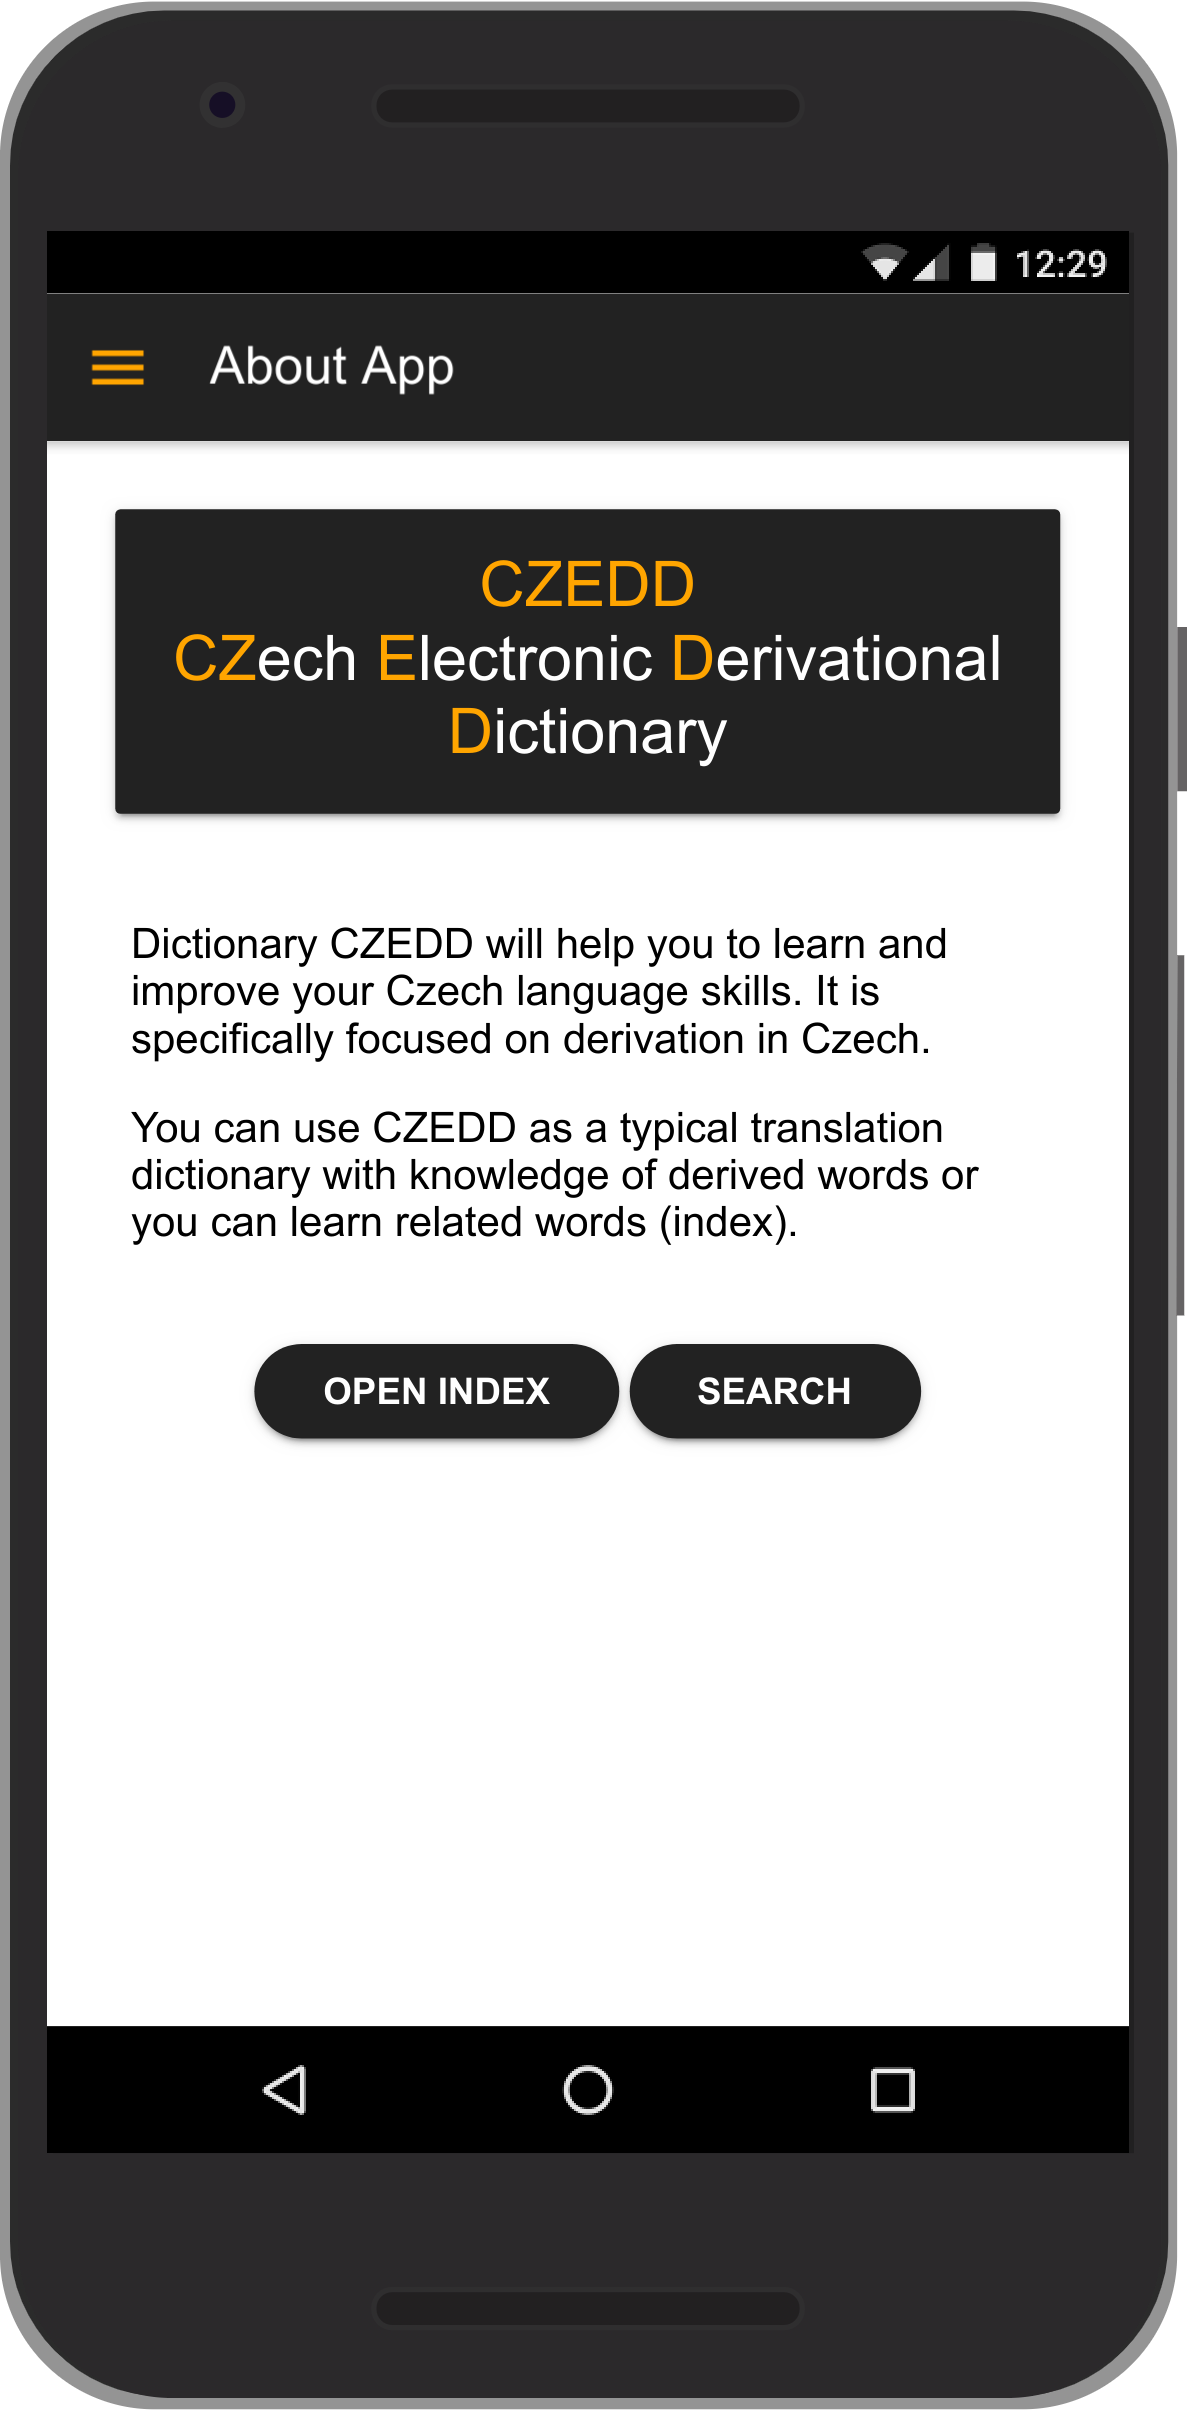
\includegraphics[width=0.9\textwidth]{1-1}
  \end{subfigure}
  \hfill
  \begin{subfigure}[b]{0.45\textwidth}
    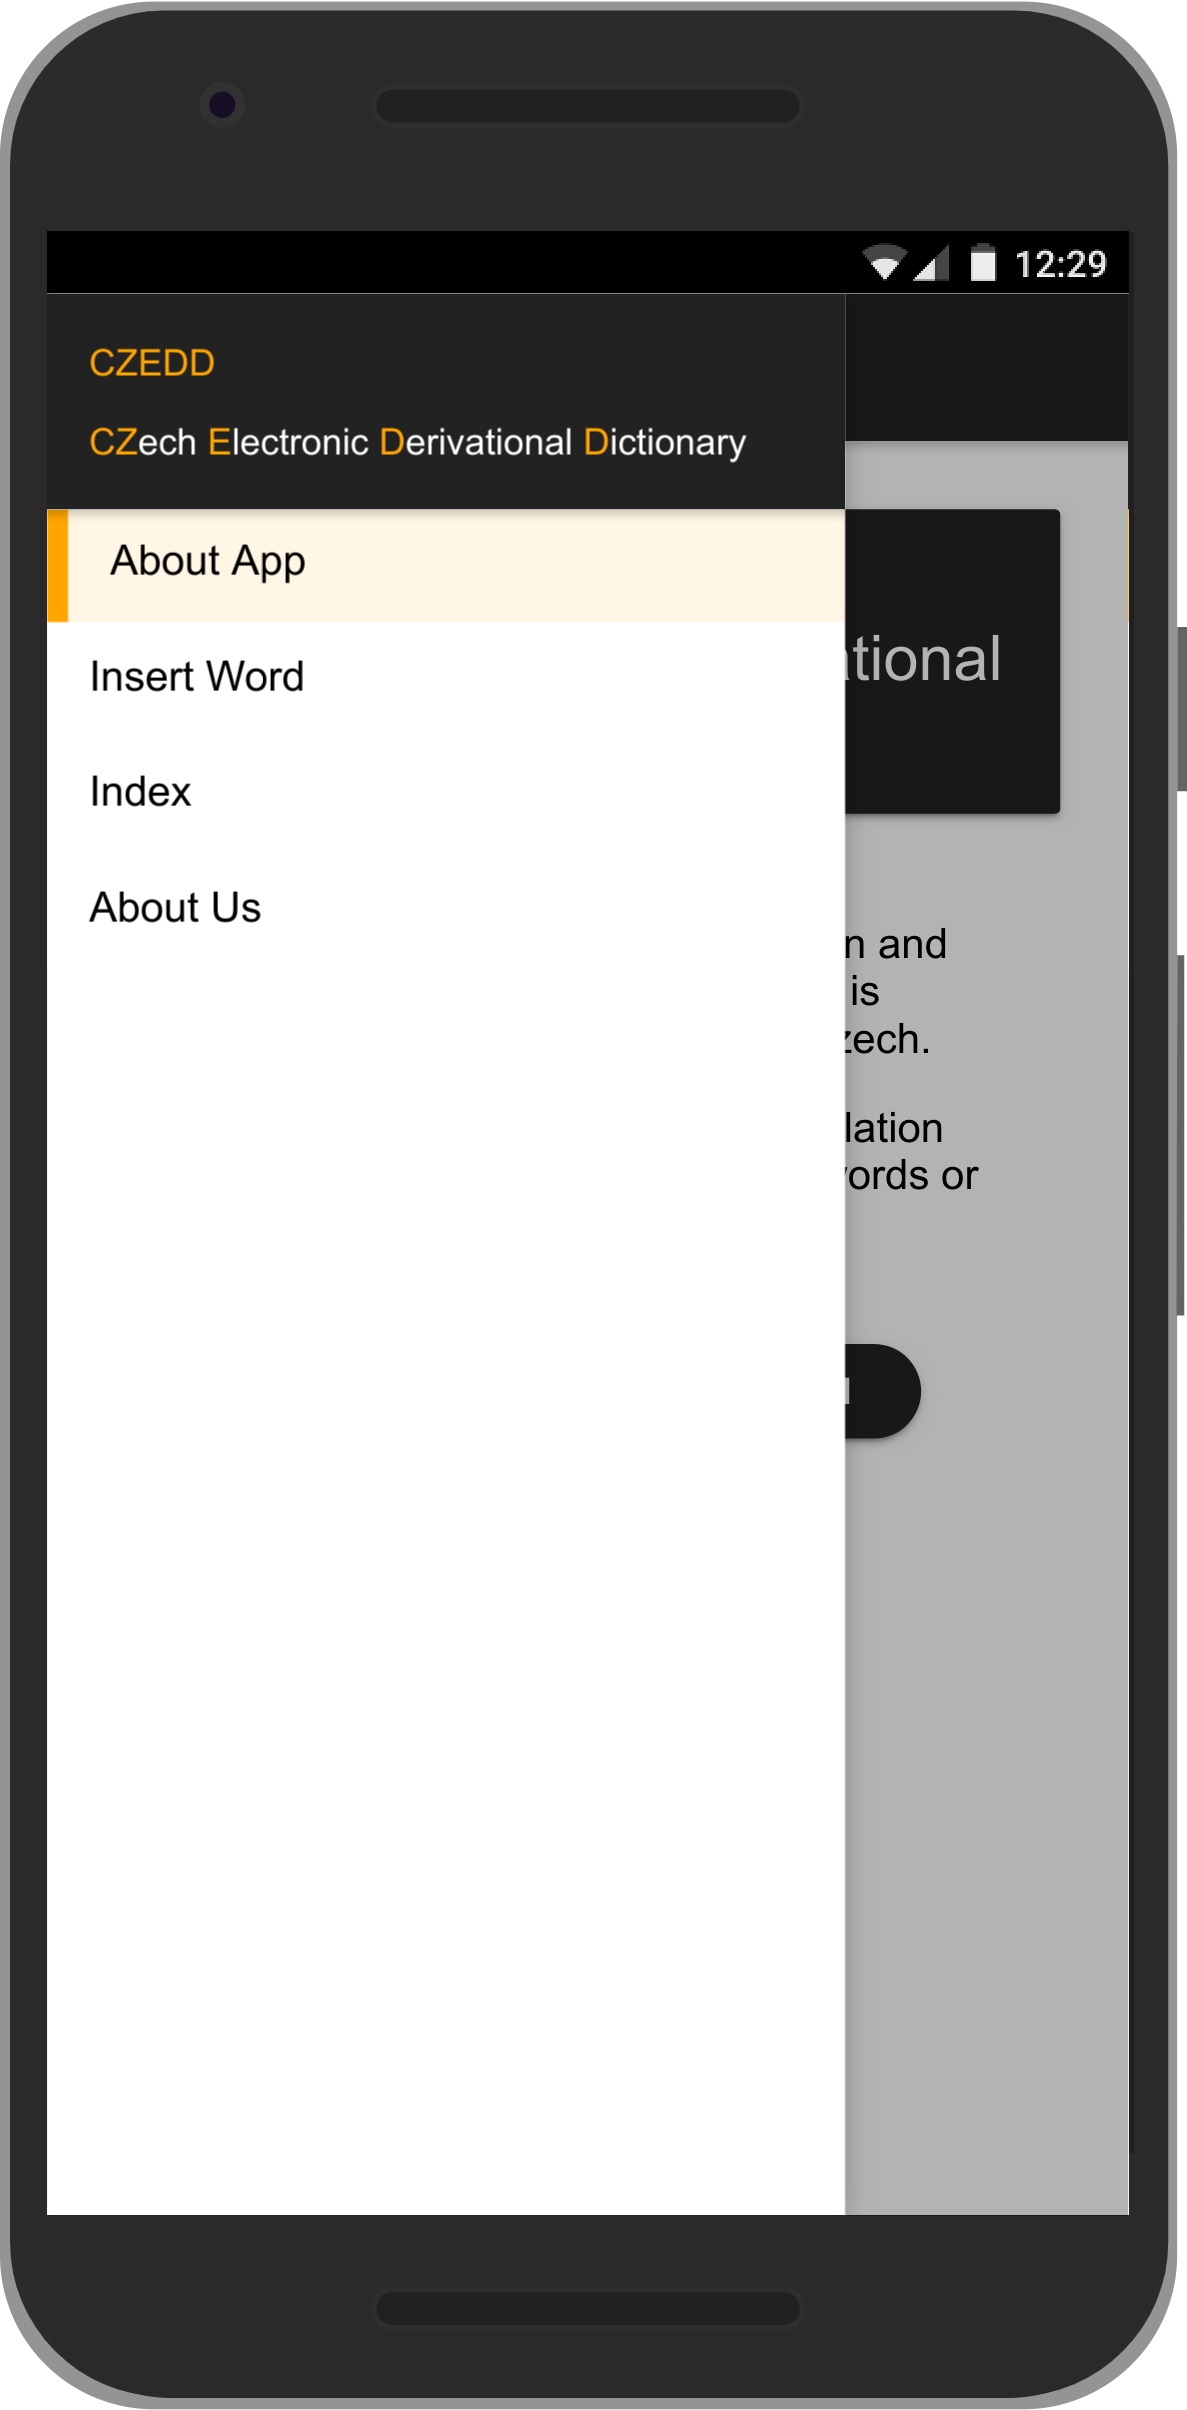
\includegraphics[width=0.9\textwidth]{1-2}
  \end{subfigure}
  \caption{Úvodní stránka a~navigační menu}
  \label{1}
\end{figure}

Nejdůležitějším prvkem celého uživatelského rozhraní je přístup k~hlavní
funkcionalitě \emph{insert word}. Domníváme se, že právě zde musí dojít
k~co nejpříjemnějšímu uživatelskému zážitku, protože na tomto místě
dochází k~uspokojení, či neuspokojení potřeb uživatele vzhledem
k~aplikaci.

S~ohledem na výše zmíněné, je výchozím stavem prázdné textové pole,
které očekává vstup od uživatele. Po zadání jednotlivých znaků obrazovka
dynamicky zobrazuje pouze ta slova z~rejstříku zpracovaných slov, která
začínají podřetězcem zadaného slovního tvaru (viz obrázek \ref{2}).
A~právě přes tato vyselektovaná slova se lze dostat k~výslednému
slovníkovému heslu.

\begin{figure}[ht]
  \begin{subfigure}[b]{0.3\textwidth}
    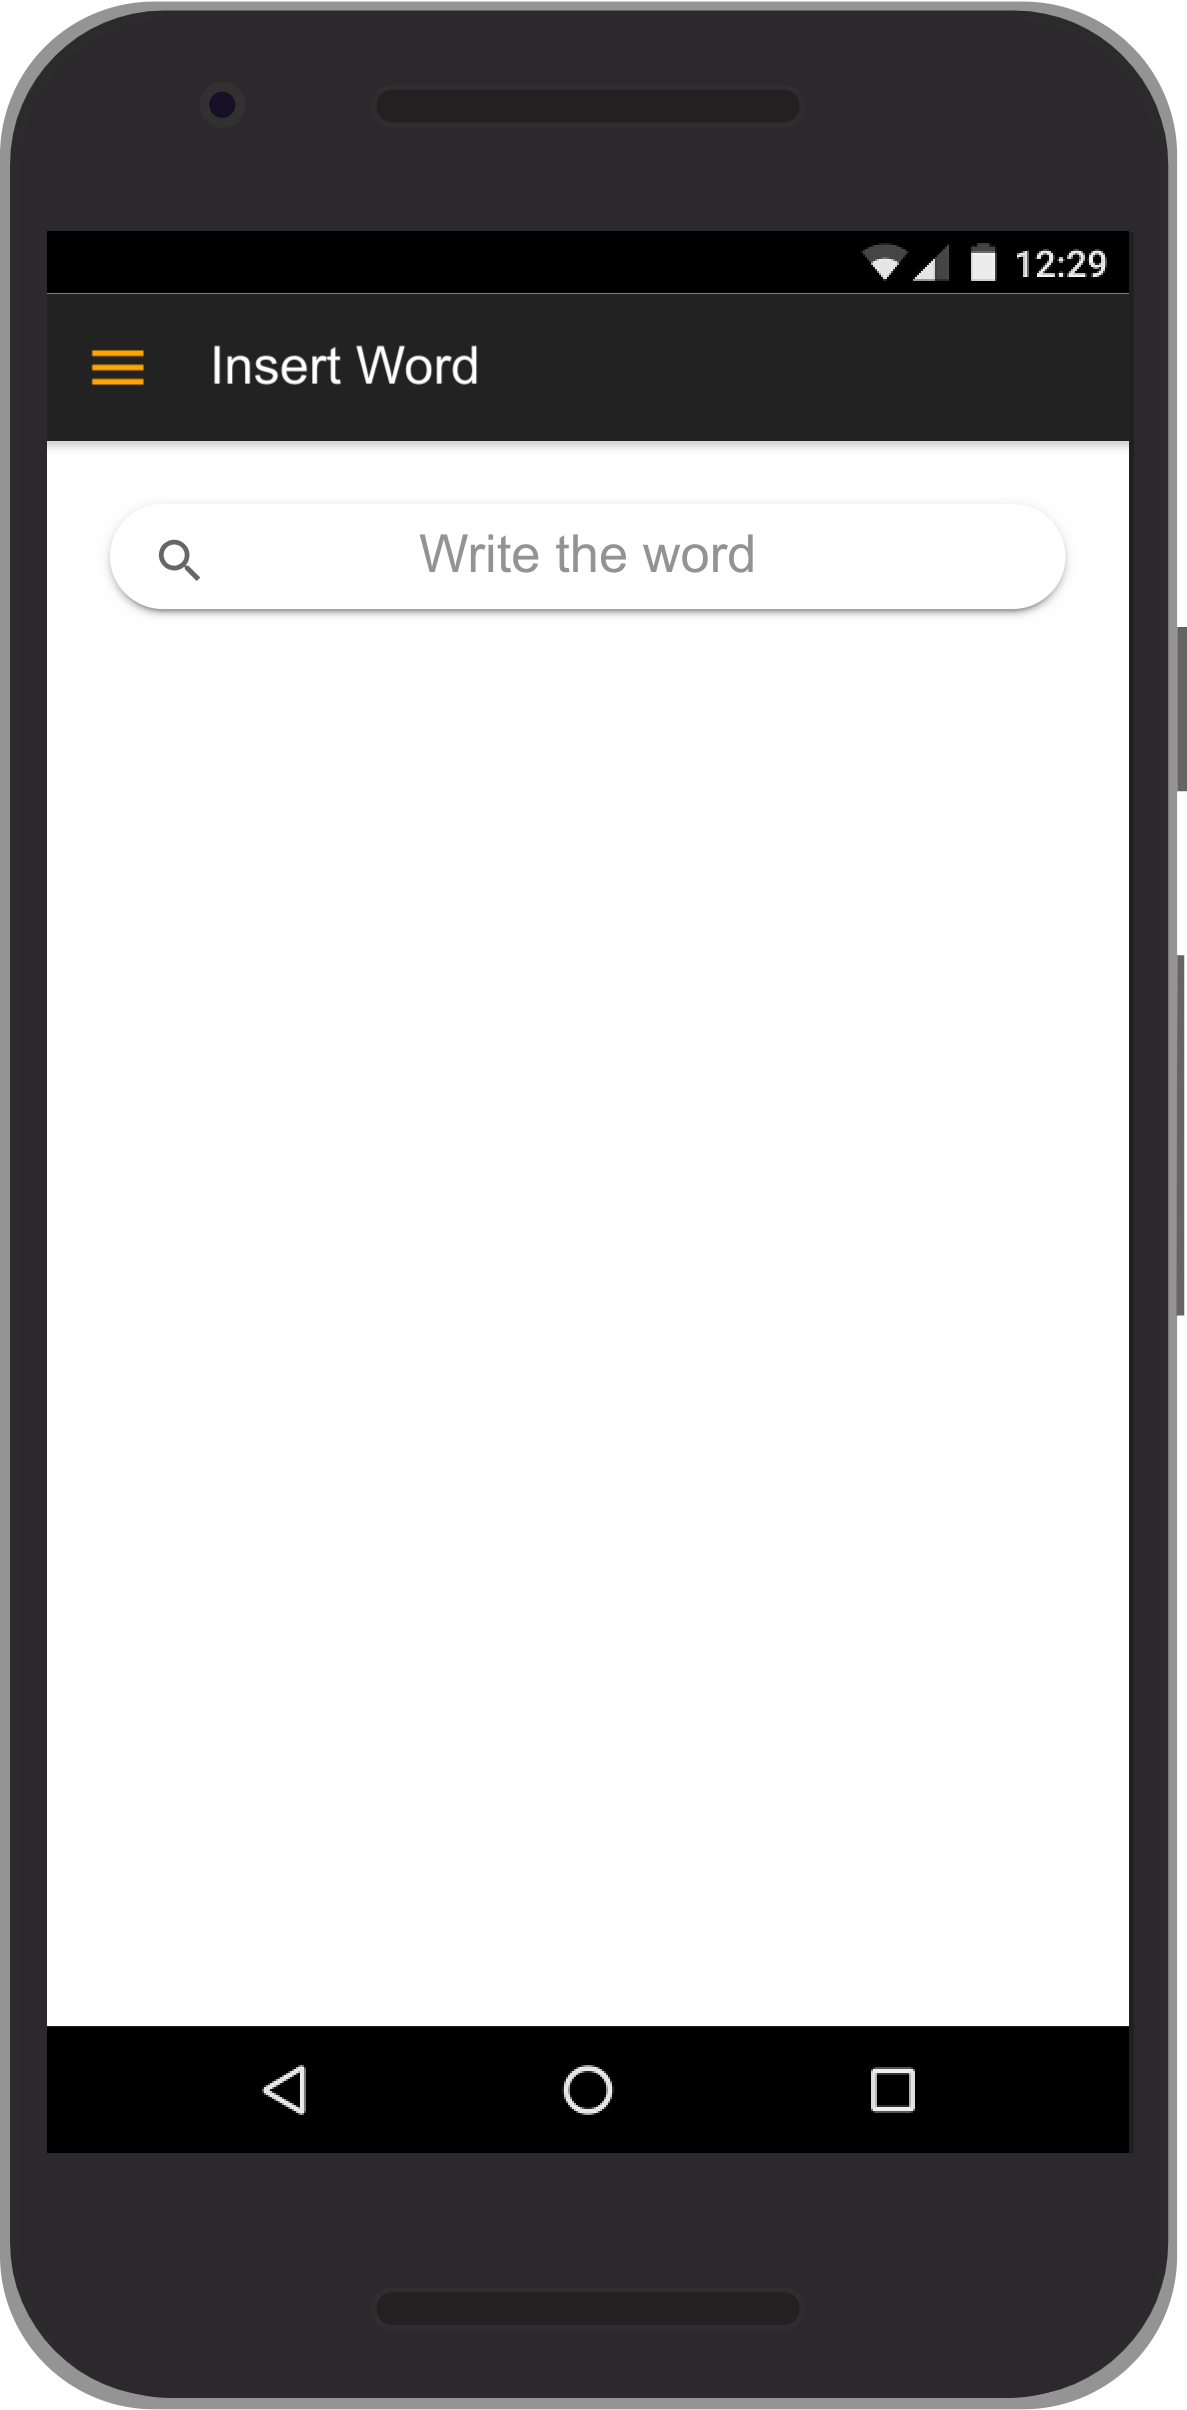
\includegraphics[width=\textwidth]{2-1}
  \end{subfigure}
  \hfill
  \begin{subfigure}[b]{0.3\textwidth}
    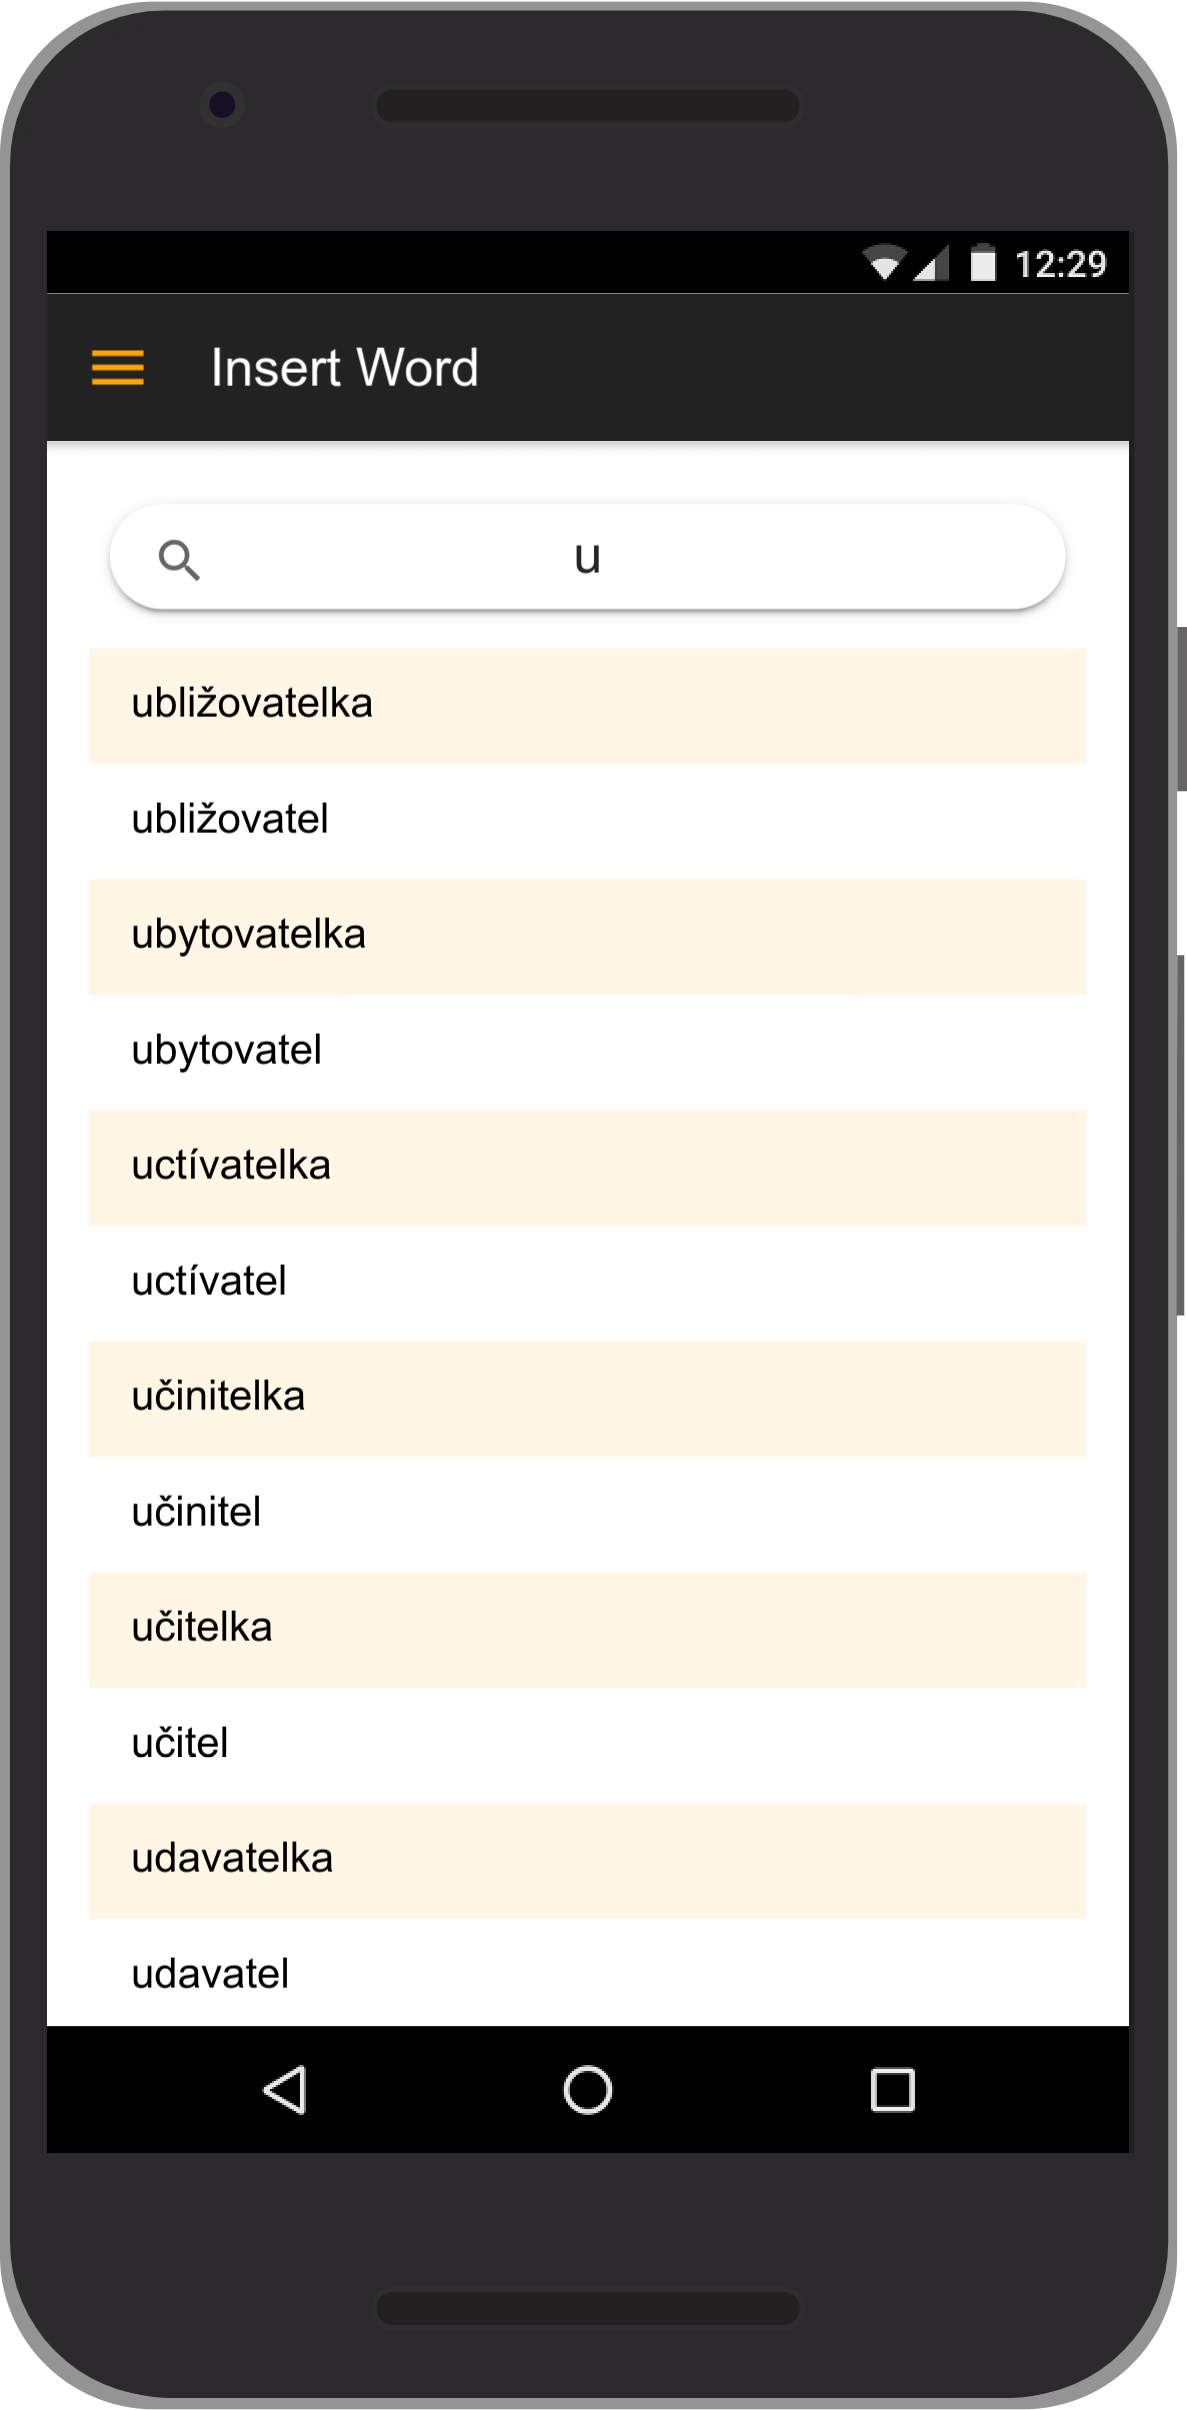
\includegraphics[width=\textwidth]{2-2}
  \end{subfigure}
   \hfill
  \begin{subfigure}[b]{0.3\textwidth}
   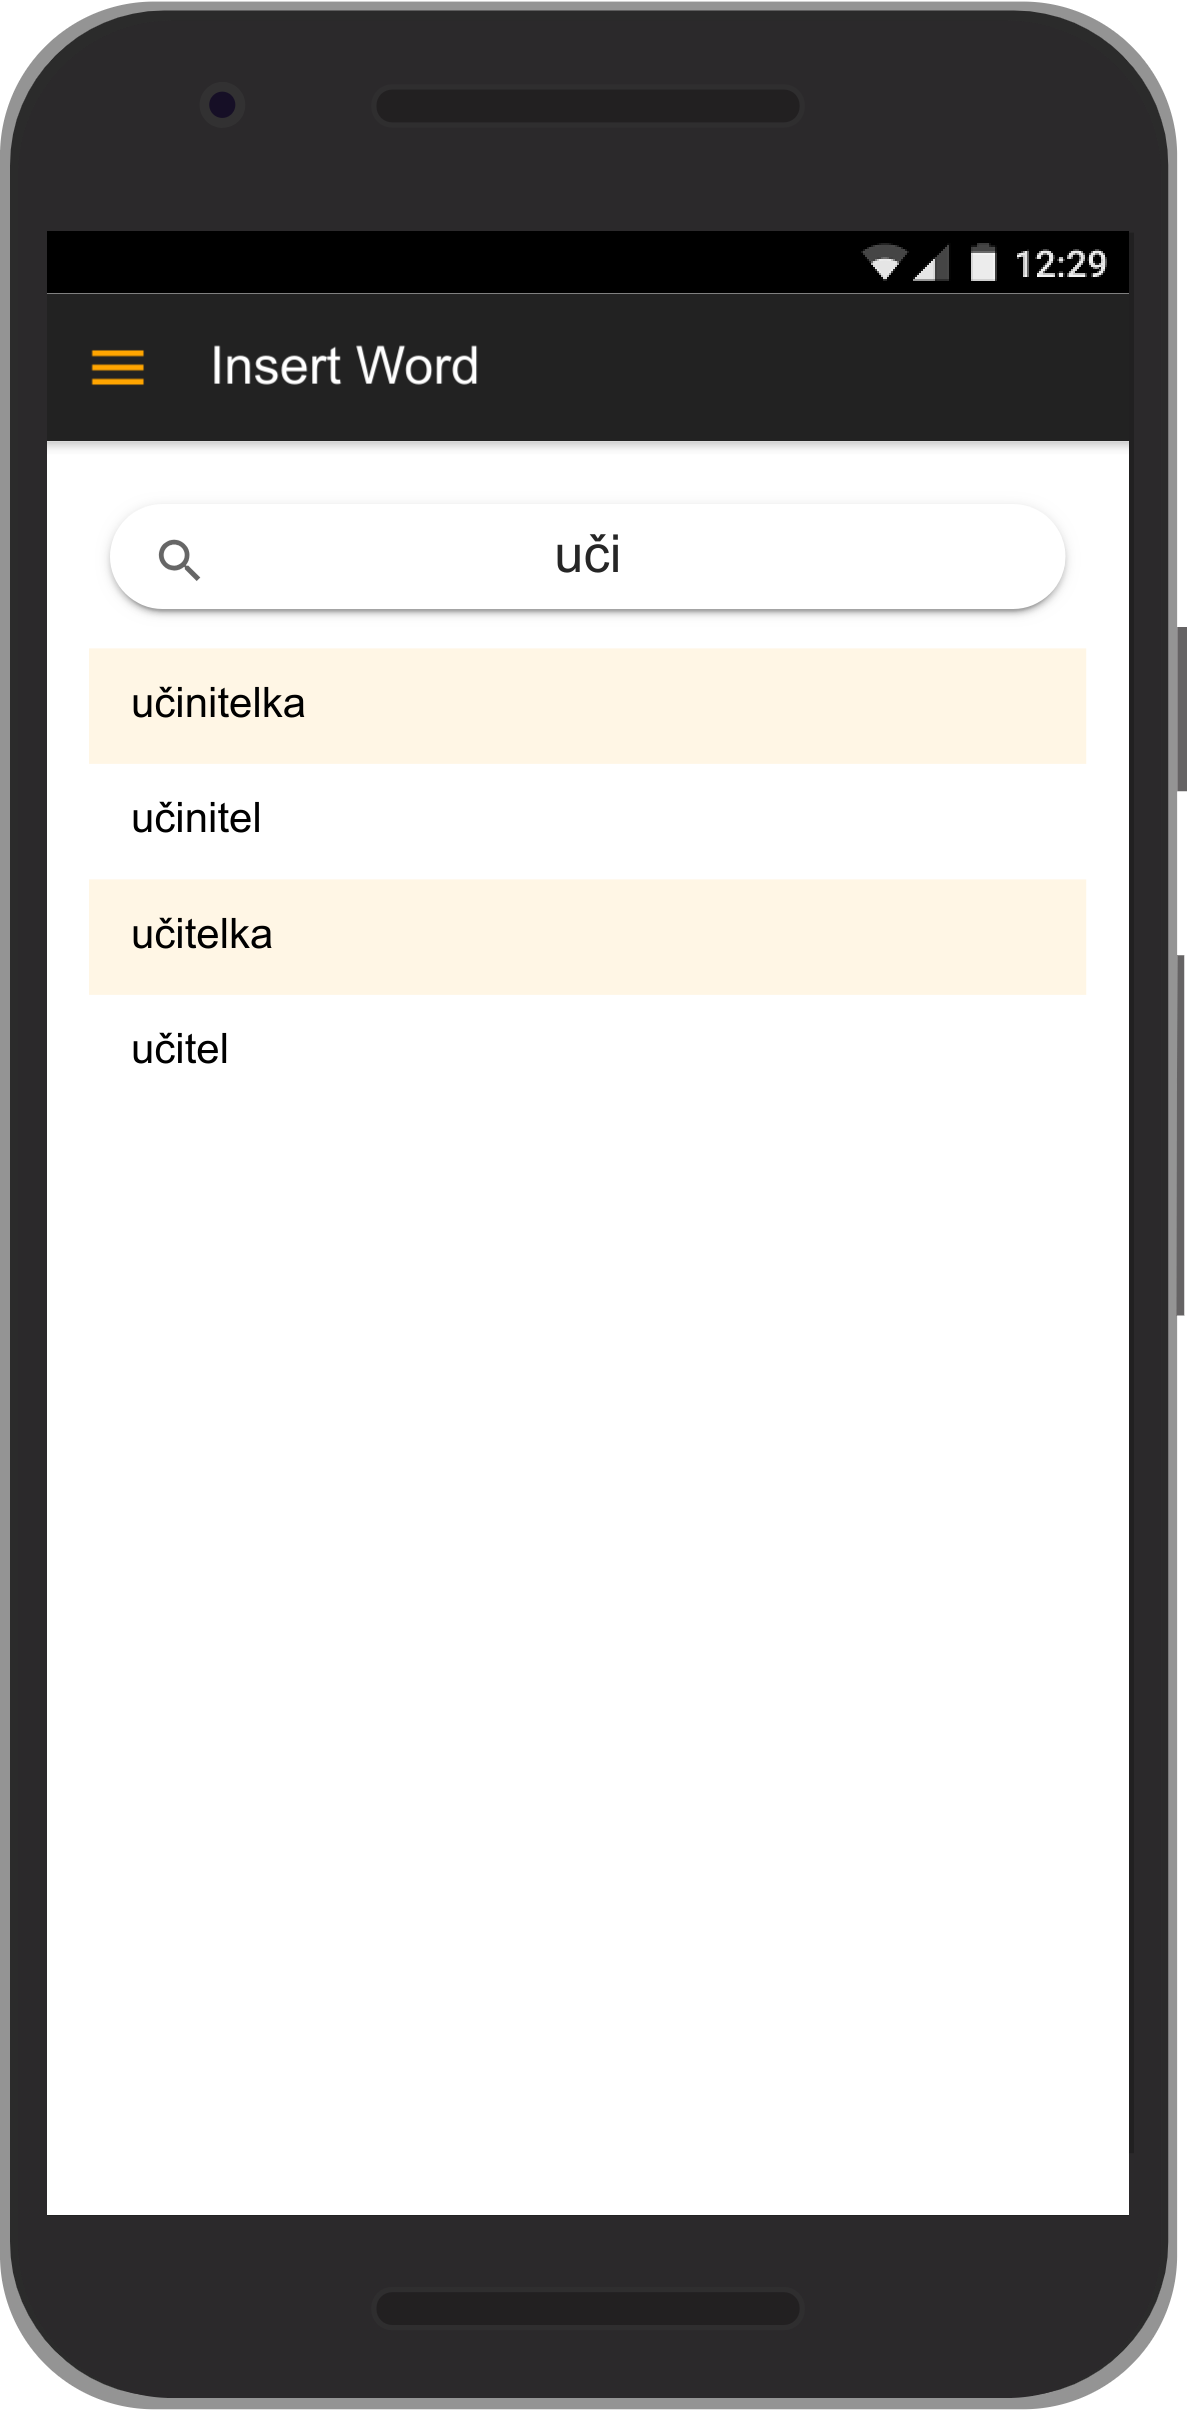
\includegraphics[width=\textwidth]{2-3}
  \end{subfigure}
  \caption{Proces zadávání vstupního slova}
  \label{2}
\end{figure}

Samotné slovníkové heslo je zobrazeno formou tří na sobě nezávislých
karet (viz obrázek \ref{3}), z~nichž každá obsahuje určité lingvistické
informace o~derivovaném výrazu (viz \ref{slovnuxedkovuxe9-heslo}).
V~případě, kdy je heslo vytvořeno na základě slova vybraného z~rejstříku
zpracovaných slov, může uživatel využít zobrazené navigační šipky (po
kliknutí na textové pole), jež ho vrátí zpět na určité místo
v~rejstříku.

\begin{figure}[ht]
  \begin{subfigure}[b]{0.45\textwidth}
    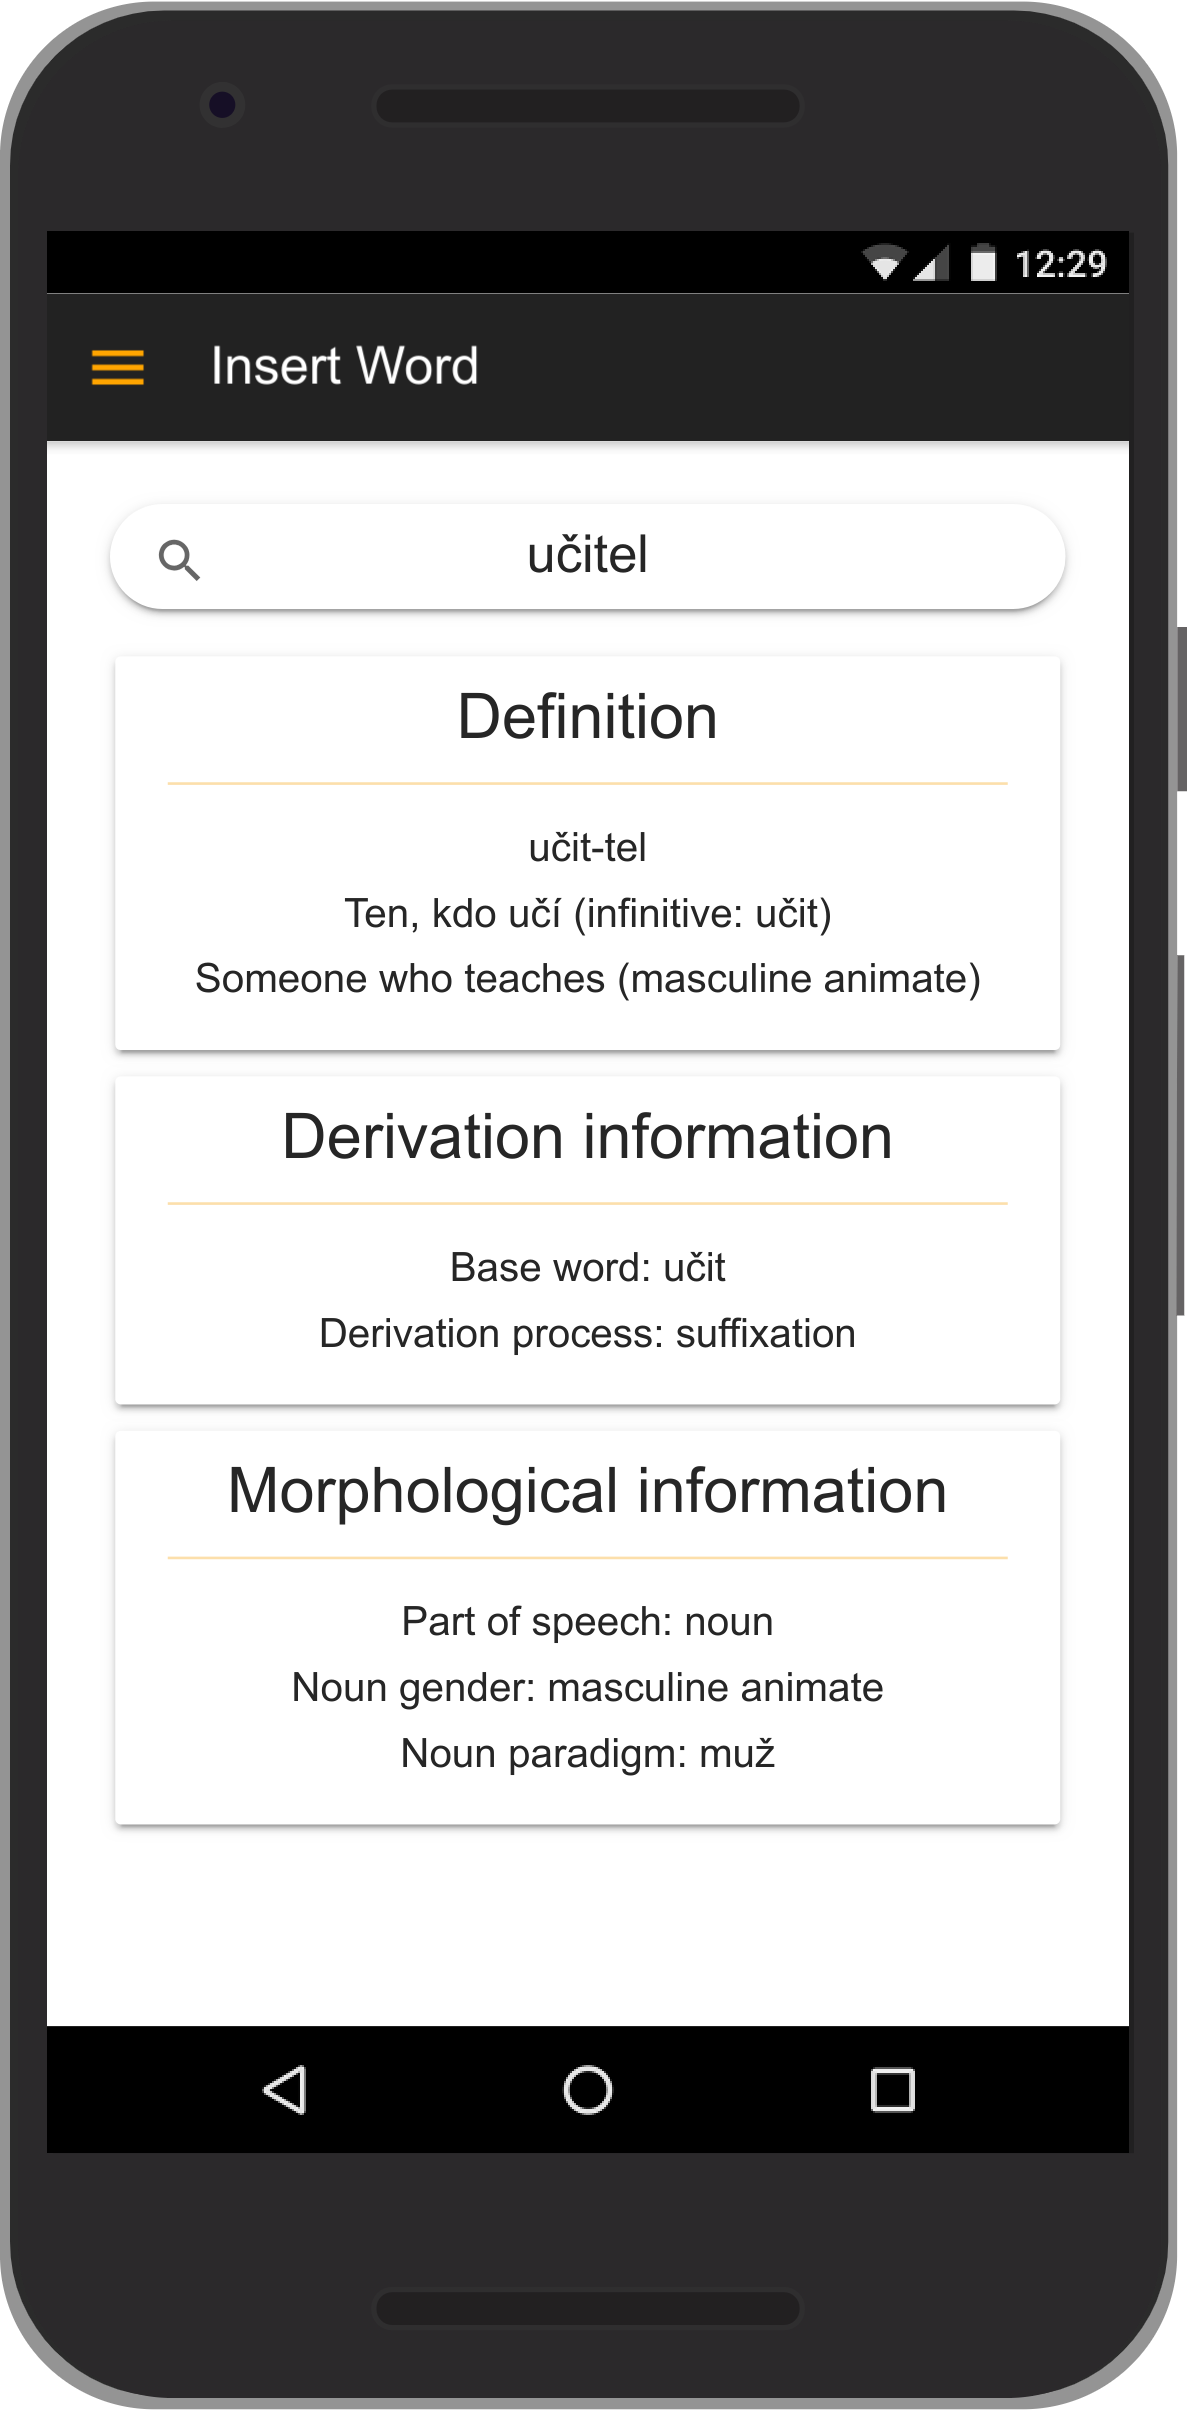
\includegraphics[width=0.9\textwidth]{3-1}
  \end{subfigure}
  \hfill
  \begin{subfigure}[b]{0.45\textwidth}
    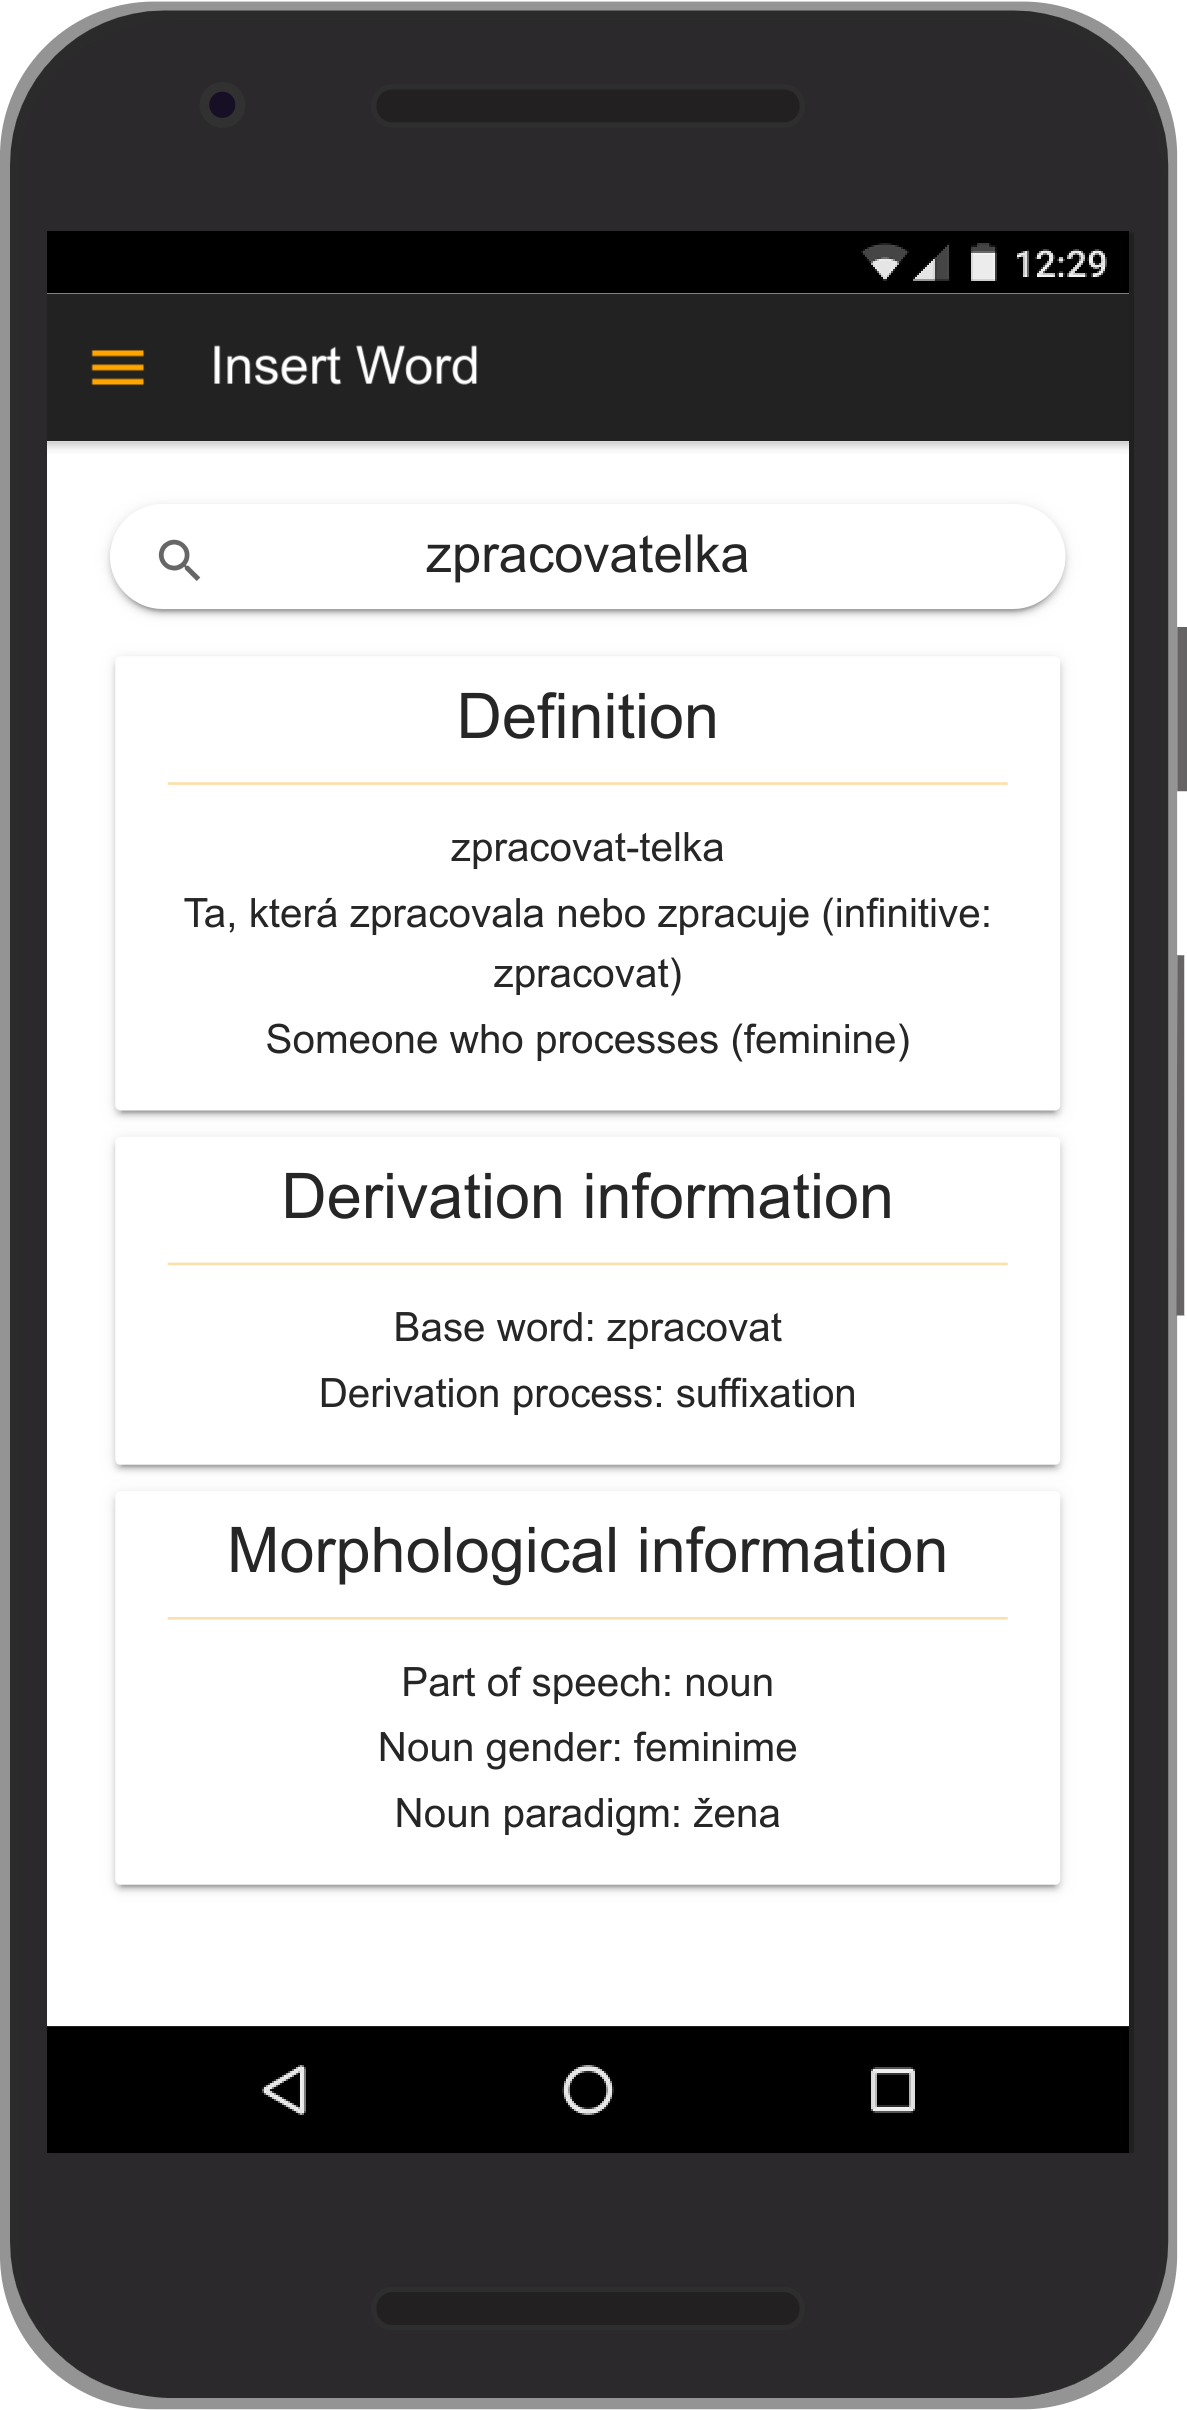
\includegraphics[width=0.9\textwidth]{3-2}
  \end{subfigure}
  \caption{Slovníková hesla}
  \label{3}
\end{figure}

Rejstřík zpracovaných slov je řazen abecedně a~obsahuje úplný seznam
slov (viz obrázek \ref{4}), která spadají do zpracovaných slovotvorných
typů. Jak bylo výše naznačeno, prostřednictvím rejstříku může uživatel
taktéž přistoupit k~vygenerování určitého slovníkového hesla.

Zbývají obrazovka je už jen marginální informační stránka týkající se
autorů, jež není pro popis návrhu uživatelského rozhraní nijak důležitá.

\begin{figure}[ht]
  \begin{subfigure}[b]{0.45\textwidth}
    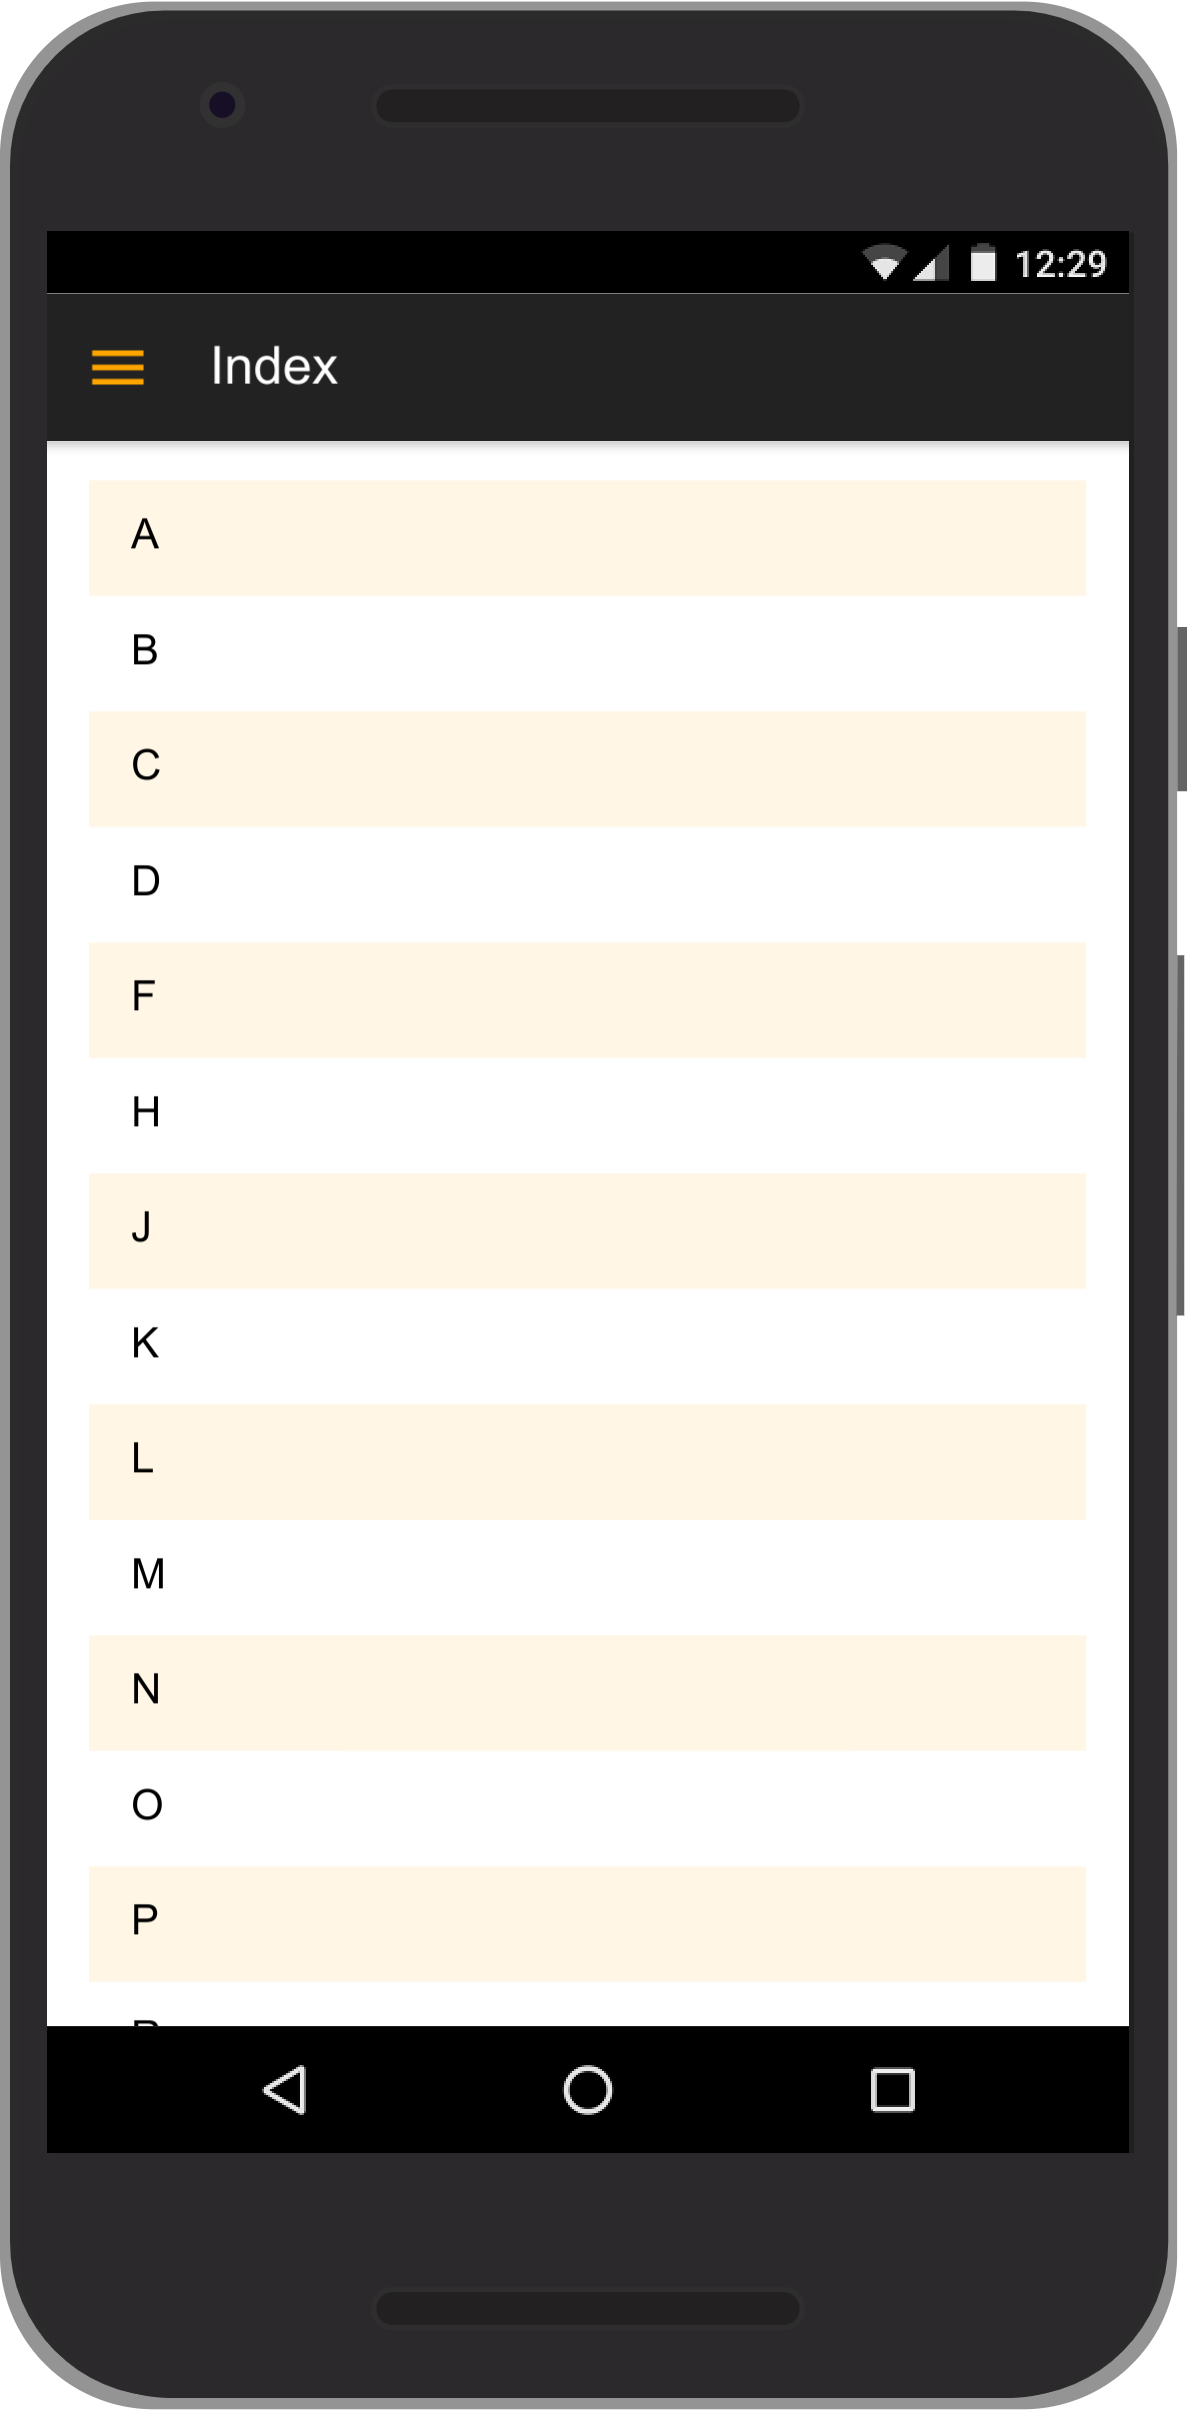
\includegraphics[width=0.9\textwidth]{4-1}
  \end{subfigure}
  \hfill
  \begin{subfigure}[b]{0.45\textwidth}
    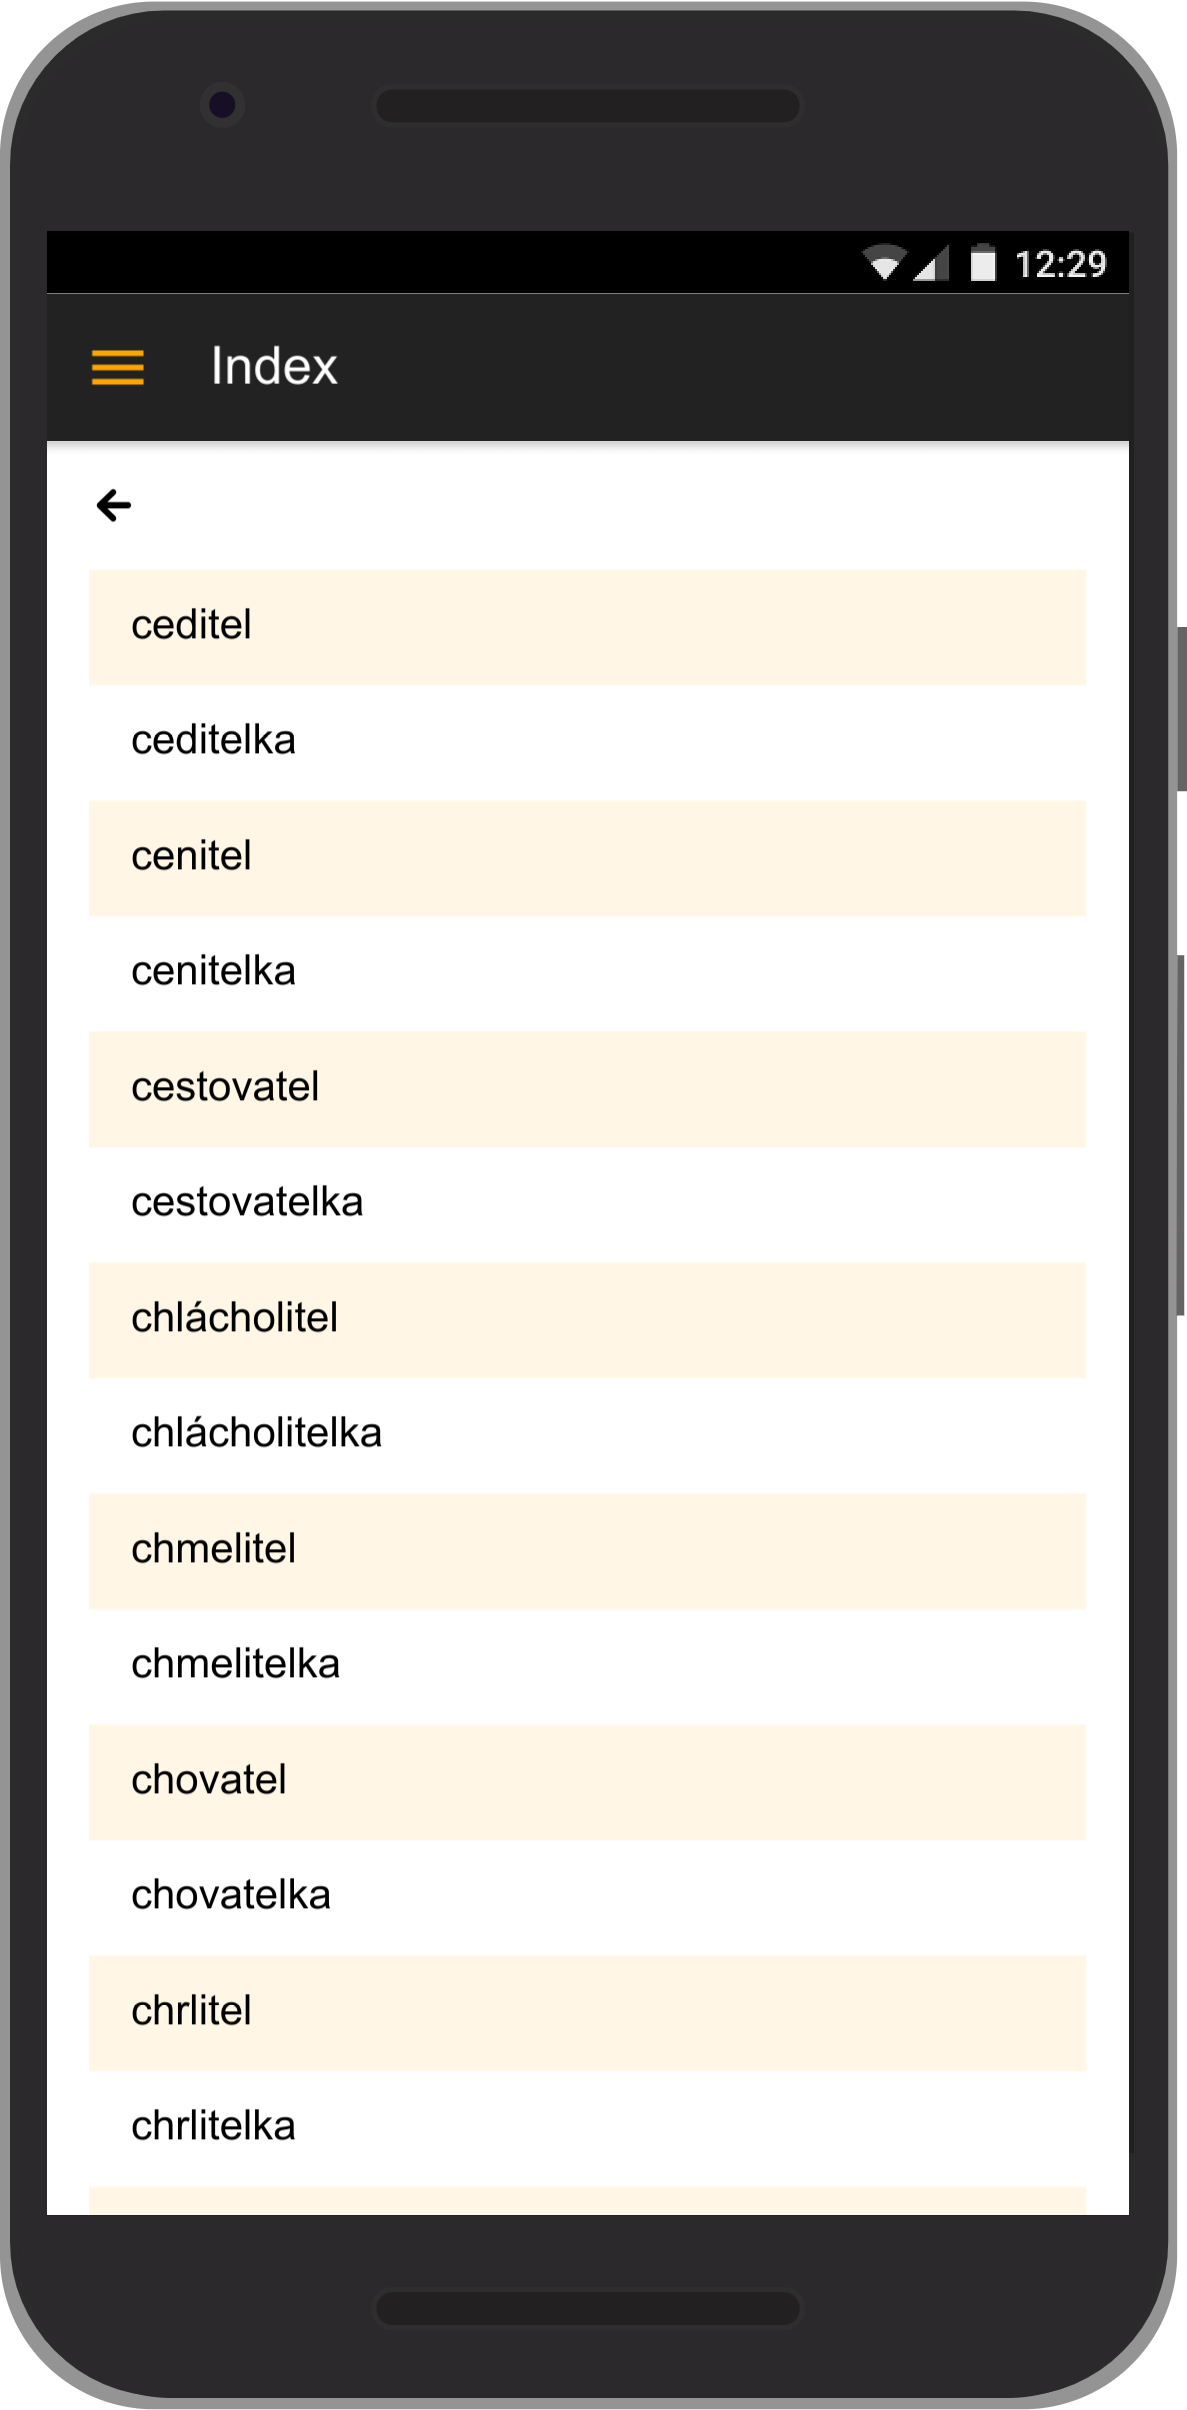
\includegraphics[width=0.9\textwidth]{4-2}
  \end{subfigure}
  \caption{Rejstřík zpracovaných slov}
  \label{4}
\end{figure}

\hypertarget{implementace-aplikace}{%
\section{Implementace aplikace}\label{implementace-aplikace}}

V~poslední kapitole si popíšeme architekturu předkládané aplikace spolu
s~její hlavní funkcionalitou \emph{insert word.}

\hypertarget{architektura}{%
\subsection*{Architektura aplikace}\label{architektura}}

Mobilní aplikace se skládá z~pěti hlavních stránek (komponent), jde o:

\begin{itemize}
\tightlist
\item
  vysouvací menu;
\item
  úvodní obrazovku s~informacemi o~aplikaci;
\item
  stránku s~funkcionalitou \emph{insert word};
\item
  rejstřík se zpracovanými slovy;
\item
  stránku s~informacemi o~autorech.
\end{itemize}

\hypertarget{insert word}{%
\subsection*{Alogritmus funkcionality insert word}\label{insert word}}

Implementačně nejkomplexnější je komponenta s~funkcionalitou
\emph{insert word}, proto se na ní v~následující části důkladněji
zaměříme a~pro demonstraci použitého algoritmu použijeme přiložené
schéma (viz obrázek \ref{algoritmus}). Pro větší přehlednost jsou na
diagramu modře zvýrazněny komponenty, žlutou barvou služby, zeleně
interní uložiště s~daty a~červeně pak hlavní funkce (ty se dále větví do
menších podfunkcí, jejichž popis není pro účely tohoto popisu klíčový).

\begin{figure}[ht]   
    \centering
    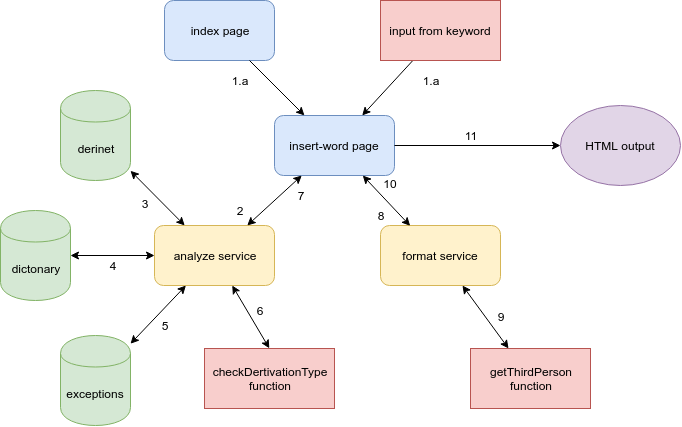
\includegraphics[width=.9\textwidth]{algoritmus}  
    \caption{Algoritmus funkcionality insert word}
    \label{algoritmus}
 \end{figure}

V~prvé řadě musí aplikace nějakým způsobem získat vstup pro následnou
analýzu, existují dva způsoby, jak k~tomu docílit -- v~případě kroku 1.a
je za vstup považováno takové slovo, které bylo vybráno v~rámci
komponenty \emph{index}, tedy je vstupní slovo vybráno na stránce
s~rejstříkem zpracovaných slov. Druhou možností (1.b) je zadat slovo ručně
prostřednictvím funkce \emph{fromUser} z~textového pole, v~takovém
případě se po zadání prvního písmena (a~následně dalších znaků)
vyselektují všechna slova z~rejstříku, která začínají zadaným
podřetězcem.

V~okamžiku, kdy je vybráno vstupní slovo, je tento řetězec zaslán do
služby \emph{analyze} (2), která řeší všechny záležitosti týkající se
derivační sítě DeriNet a~překladu. V~této službě se při jejím volání
inicializuje objekt, který bude cílovým výstupem této služby -- tento
objekt nazýváme \emph{infoBase} a~skládá se z~několika atributů:

\begin{itemize}
\tightlist
\item
  vstup v~českém jazyce (při inicializaci je za jeho hodnotu přiřazeno
  vstupní slovo);
\item
  vstup v~anglickém jazyce (při inicializaci je spuštěn automatický
  překlad);
\item
  slovotvorný typ (tento a~zbytek atributů zůstávají při inicializaci
  prázdné);
\item
  prefigovanost;
\item
  prefix;
\item
  derivační proces;
\item
  rod;
\item
  derivační cesta.
\end{itemize}

Při inicializaci se souběžně načítají data z~interního uložiště, která
jsou následně zkonvertována do použitelného datového formátu (3, 4, 5),
konkrétně jde o~databázi DeriNet, česko-anglický slovník
Glosbe\footnote{https://glosbe.com/ -- jedná se o~open-source projekt pod licencí CC-BY-SA z~něhož byla vyextrahována data pro naše použití.}
a~seznam výjimek (viz kapitola
\ref{zpracovanuxe9-slovotvornuxe9-sufixy}).

Dalším krokem je postupné procházení derivační sítě DeriNet, z~níž
potřebujeme vyextrahovat výše zmíněné lingvistické informace, procházíme
tedy derivační řetězec směrem od slova vstupního k~jeho slovu
základovému do té chvíle, než se zamění slovní druh, pak přistupujeme
k~volání funkce \emph{checkDertivationType} (6). Ta nám porovná řetězce
obou slov a~určí, o~jaký se jedná derivační proces a~slovotvorný typ.
Dále určuje algoritmus z~celého derivačního řetězce prefigovanost
(popřípadě zjišťuje o~jaký prefix se přesně jedná), zaznamená si rod
vstupního slova (ve výjimkách máme tedy v~případě slovotvorného sufixu
\emph{-tel} taková slova, která jsou neživotnými maskuliny) a~ukládá si
základové slovo spolu s~jeho anglickým ekvivalentem (u~českých
odvozených slov ve slovníku často překlad chybí). Posléze služba
\emph{analyze} vrací již vyplněný objekt \emph{infoBase} zpátky do
komponenty \emph{insert-word}, vrácený objekt může vypadat například
takto:

\begin{verbatim}
1.  czechInput:  "zpracovatel"
2.  czechParent:  "zpracovat"
3.  derProcess:  "suffixation"
4.  derivType:  "tel"
5.  derivationPath:  (2) [{…},  {…}] // derivační řetězec
6.  englishInput:  ""
7.  englishParent:  "processes"
8.  gender:  "M"
9.  isPrefig:  true
10. prefix:  "z"
\end{verbatim}

Nyní se dostáváme do kroku č. 8, kdy je objekt \emph{infoBase} předán
druhé službě s~názvem \emph{createDefiniton}, jejímž účelem je vytvořit
samotné slovníkové heslo do formy objektu \emph{definiton}. Jednotlivé
části jsou zpracovány separátně, a~to jednak z~důvodu přehlednosti kódu,
ale taktéž z~ryze praktické příčiny, tedy aby s~výsledným objektem byla
co nejjednodušší manipulace na úrovní HTML šablony.

Na začátku inicializujeme obecnou slovotvornou definici podle rodu ze
vstupního objektu \emph{infoBase} a~poté přistupujeme k~funkci
\emph{getThirdPerson} (9), v~rámci které vytváříme slovesnou formu ve
třetí osobě podle lingvistických pravidel popsaných v~kapitole
\ref{slovotvornuxe1-definice}.

Následně dotvoříme derivační a~morfologickou informaci z~poznatků
získaných ze služby \emph{analyze} a~vracíme objekt \emph{definiton}
zpět do komponenty \emph{insert-word} (10). Pokud je vrácen objekt
správného typu, je HTML šabloně umožněno skrze direktivy frameworku
Angular přistoupit k~jednotlivým častém definice a~vykreslit je do
označených míst v~šabloně (11).

Výhoda tohoto objektového přístupu je taková, že se na jednotlivých
jasně otypovaných místech v~kódu provádí pouze jeden specifický úkol,
a~tím je do určité míry zajištěna robustnost celkové aplikace, kdy je při
výpadku jedné služby/funkce jednoduché lokalizovat místo chyby.

\hypertarget{zuxe1vux11br}{%
\chapter*{Závěr}\label{zaver}
\addcontentsline{toc}{chapter}{Závěr}}

Cílem této práce bylo navrhnout a~implementovat elektronický slovník
s~definicemi založenými na derivačních rysech slovotvorně motivovaných
slov. Aplikaci se podařilo implementovat dle zadaných požadavků, její
instalace a~testování proběhlo na mobilním zařízení s~operačním systémem
Android ve verzi 7.

Vzhledem ke složitosti slovotvorného systému českého jazyka jsou
v~aktuální verzi zpracována slova spadající do slovotvorných typů
\emph{-tel} a~\emph{-telka}. U~těchto slov byla navrhnuta lingvistická
pravidla, která slouží pro vytváření slovotvorných definic. S~ohledem na
cílovou skupinu (cizinci studující češtinu jako druhý jazyk) byl
vyhledán dvojjazyčný česko-anglický slovník, pomocí kterého jsou
slovotvorné definice kompletně lokalizovány v~anglickém jazyce.

V~budoucím vývoji aplikace se počítá s~navýšením počtu zpracovaných
slovotvorných typů (další v~pořadí je typ \emph{-ista}). Z~hlediska
uživatelského prostředí by se bylo dále vhodné zaměřit na implementaci
autentifikačního systému, v~rámci kterého by si tak uživatel mohl
ukládat již naučená slova (případně slovotvorné typy) do své vlastní
profilové stránky. Taktéž se do budoucna počítá s~propojením mobilní
aplikace s~webovou verzí, která bude svými vlastními funkcionalitami
předkládanou aplikaci doplňovat.

Cíle této práce byly splněny a~její výstupy by tak měly být rozšířeny
v~rámci případného navazujícího aplikovaného výzkumu.

\clearpage

\pagestyle{plain}

\addcontentsline{toc}{chapter}{Seznam literatury}
\begin{spacing}{1.05}
\printbibliography[title={Seznam literatury}]
\end{spacing}

\end{document}